\documentclass[11pt,letterpaper,oneside]{report}
\usepackage[margin=1.1in]{geometry}
\usepackage{amsmath,amsthm}
\usepackage{newtxtext,newtxmath}
\usepackage{microtype}
\usepackage{graphicx}
\usepackage{booktabs}
\usepackage{tabularx}
\usepackage{xltabular}
\usepackage{enumitem}
\usepackage{xcolor}
\usepackage[most]{tcolorbox}
\usepackage{tikz}
\usetikzlibrary{positioning,arrows.meta}
\usepackage{listings}
\usepackage[hidelinks]{hyperref}
\usepackage{titlesec}
\usepackage{fancyhdr}

\graphicspath{{../../results/figures/paper/}}
\setlist{itemsep=2pt,topsep=4pt}
\setlength{\parskip}{5pt}
\setlength{\parindent}{0pt}
\linespread{1.08}
\setlength{\emergencystretch}{2.5em}

\titleformat{\chapter}[display]{\normalfont\bfseries\Large}{\large Chapter \thechapter}{4pt}{\LARGE}
\titlespacing*{\chapter}{0pt}{-10pt}{18pt}
\pagestyle{fancy}
\fancyhf{}
\fancyhead[L]{\small\itshape Reader's companion}
\fancyhead[R]{\small\itshape \leftmark}
\fancyfoot[C]{\small\thepage}
\renewcommand{\chaptermark}[1]{\markboth{#1}{}}

\definecolor{paperbg}{HTML}{F2F1EC}
\definecolor{plainbg}{HTML}{EAF1FB}
\definecolor{plainfr}{HTML}{2A78D6}
\definecolor{exbg}{HTML}{E8F5EE}
\definecolor{exfr}{HTML}{13804F}
\definecolor{askbg}{HTML}{FBF2DF}
\definecolor{askfr}{HTML}{B7791F}
\definecolor{whybg}{HTML}{F1EEF9}
\definecolor{whyfr}{HTML}{6250D6}
\definecolor{ancblue}{HTML}{2A78D6}
\definecolor{sibor}{HTML}{EB6834}
\definecolor{offgray}{HTML}{C3C2B7}

\tcbset{boxsep=3pt,left=6pt,right=6pt,top=4pt,bottom=4pt,arc=2pt,breakable,fonttitle=\bfseries\small,coltitle=black}
\newtcolorbox{paper}{colback=paperbg,colframe=paperbg!70!black,title=From the paper,colbacktitle=paperbg!85!black,fontupper=\small\itshape}
\newtcolorbox{plain}{colback=plainbg,colframe=plainfr,title=In plain words,colbacktitle=plainbg!80!plainfr}
\newtcolorbox{example}[1][]{colback=exbg,colframe=exfr,title={With real numbers#1},colbacktitle=exbg!80!exfr}
\newtcolorbox{ask}{colback=askbg,colframe=askfr,title=If an examiner asks,colbacktitle=askbg!80!askfr}
\newtcolorbox{why}{colback=whybg,colframe=whyfr,title=Why it was done this way,colbacktitle=whybg!80!whyfr}

\lstset{basicstyle=\ttfamily\small,columns=fullflexible,keepspaces=true,frame=single,rulecolor=\color{black!25},backgroundcolor=\color{paperbg},xleftmargin=4pt,xrightmargin=4pt,breaklines=true}

\newcommand{\A}{A(a)}
\newcommand{\Sib}{S(a)}
\newcommand{\anc}{\mathrm{anc}}
\newcommand{\full}{\mathrm{full}}
\newcommand{\win}{\mathrm{win}}
\newcommand{\term}[1]{\textbf{#1}}

\begin{document}

\begin{titlepage}
\centering
\vspace*{1.6in}
{\Huge\bfseries The Only Path That Matters?\par}
\vspace{10pt}
{\Large Ancestor-Only Context Selection in Branched LLM Conversations\par}
\vspace{28pt}
{\LARGE A reader's companion\par}
\vspace{10pt}
{\large Every term, formula, decision and figure, explained line by line\par}
\vspace{48pt}
{\large Prepared for Okechukwu Zeal Achonu\par}
\vfill
{\small Companion to the paper draft \texttt{docs/paper/paper.pdf}. All numbers come from the frozen\\ dataset (tag \texttt{thesis-freeze-v1}) and \texttt{results/analysis/stats.txt}.\par}
\end{titlepage}

\tableofcontents
\clearpage

\chapter*{How to read this book}
\addcontentsline{toc}{chapter}{How to read this book}
\markboth{How to read this book}{}

This book walks through your paper from the first word to the last and assumes nothing. If a sentence in the paper uses a word, a symbol or a procedure, this book explains it before or right where it is used. You can read it from start to finish like a textbook, or keep it open next to the paper and look up the part you are on.

The paper is short because conference papers have to be. This book is long because it fills in everything the paper leaves out: what each term means, why each decision was made, how each number was produced, and how to read each graph.

\section*{The five kinds of box}

Five kinds of shaded box appear throughout. They always mean the same thing.

\begin{paper}
A grey box quotes the paper itself, so you always know which sentence is being explained.
\end{paper}

\begin{plain}
A blue box says the same thing in ordinary words, with no jargon.
\end{plain}

\begin{example}
A green box works through the idea with real numbers from your experiment, usually from one scenario that this book follows all the way through.
\end{example}

\begin{why}
A purple box records a decision: what was chosen, what the alternatives were, and why. These are the decisions you made months ago and may no longer remember.
\end{why}

\begin{ask}
An amber box gives a question an examiner is likely to ask at this point, with an answer you can give in your own words.
\end{ask}

\section*{The running example}

Many chapters use the same scenario, \texttt{cache-conflicting-d4-k3-early-root-00}. It is a conversation in which a developer decides to use \textbf{LRU} as the eviction policy for a product cache. Three side branches then explore other policies (LFU, ARC and FIFO) before the developer returns to the main thread and asks, ``which eviction policy did we choose?'' The correct answer is LRU. Following one scenario through every stage (building it, loading it, building the three prompts, sending them to the models, scoring the answers) is the fastest way to see how the pieces fit together.

\section*{A suggested plan}

\begin{enumerate}
\item Read Chapters 1 to 3 in one sitting. They give the whole picture and the vocabulary.
\item Read Chapter 4 (the formulas) slowly, with a pencil. Recompute the green boxes yourself.
\item Read Chapters 5 to 9 alongside the paper's Methodology and Results sections.
\item Before any meeting with your advisor or your defense, reread Chapters 10 to 12.
\end{enumerate}

\chapter{The big picture}

\section{The problem in one story}

Imagine you are building an invoicing app and you ask an AI assistant for help with the database. You decide the users table will use a particular kind of primary key. Later you wonder whether another kind would be better, so you explore it for a few messages, decide against it, and go back to what you were doing. Then you explore a third option, and abandon that too. Twenty messages later you ask: ``remind me, which key type did we settle on?''

In a normal chat app, everything you typed is one long list. When you send a new message, the app sends the model the whole list, including all the options you explored and rejected. Two things go wrong:

\begin{enumerate}
\item \textbf{Cost.} The model is paid by the amount of text it reads. Re-sending abandoned explorations on every turn wastes money, and the waste grows as the conversation gets longer.
\item \textbf{Confusion.} The rejected options are still in front of the model. It may answer with one of them, mix them together, or mention them when they no longer matter. Research shows models get less reliable as their input gets longer and noisier.
\end{enumerate}

\section{What Traceback does differently}

Traceback, the app you built, stores a conversation as a \term{tree} instead of a list. Every time you explore an alternative, you make a new \term{branch}. When you are back on your main line of thought and send a message, Traceback sends the model only the messages on the path from the very first message down to where you are now. The abandoned branches are left out. Your paper calls this \term{ancestor-only prompting}, because the messages on that path are the \emph{ancestors} of your current message.

\begin{plain}
A list-based chat shows the model your whole diary, rejected ideas included. Traceback shows the model only the pages that lead to where you are now.
\end{plain}

\section{Why this needed an experiment}

That sounds obviously better, so why test it? Because there is a simpler alternative that also saves money: just send the most recent messages, up to some size limit. This is called a \term{sliding window}, and many products do it. A sliding window is also short and cheap. So the real question is not ``is a shorter prompt better than a longer one?'' (earlier work already showed that) but:

\begin{quote}
\emph{If two prompts are the same size, does choosing the messages by their position in the tree beat choosing them by how recent they are?}
\end{quote}

That is the gap your thesis fills. The earlier branching study by Chickmagalur Nanjundappa and Maaheshwari (reference [4] in the paper) compared branching with the full history only, so it could not tell whether branching helped because the prompt was \emph{better chosen} or merely \emph{shorter}. Your experiment holds the size fixed by giving the sliding window exactly the same number of tokens as the ancestor-only prompt.

\section{The research question and the hypothesis}

\begin{paper}
This paper asks whether, at an equal token budget, selecting context by tree structure rather than by recency reduces sibling leakage (the model using facts from inactive branches), how leakage varies by sibling type, and whether answer quality on the active path is preserved.
\end{paper}

\begin{plain}
Three questions in one sentence:
\begin{enumerate}
\item With the same amount of text, does Traceback's way of choosing messages stop the model from using information from abandoned branches more often than the ``most recent messages'' way does?
\item Does that depend on what kind of information the abandoned branch contained?
\item Do the answers stay just as good?
\end{enumerate}
\end{plain}

The hypothesis predicted three things: ancestor-only uses fewer tokens than sending the whole tree; both other methods let abandoned-branch information leak into answers; and ancestor-only keeps answer quality high when the needed fact is on the current path. All three held.

\section{The answer in one paragraph}

Across 720 test conversations and three AI models, ancestor-only prompting used 62.7\% fewer tokens than sending the whole tree. It never once used information from an abandoned branch (0 of 2,160 answers). It was correct 99.9\% of the time. Sending the whole tree was almost as correct (98.6\%) but cost three times as much, used abandoned-branch details in up to a third of answers, and scored lower on quality. The equal-size sliding window was correct only 52.0\% of the time, because it throws away the \emph{oldest} messages first, which is often exactly where the important decision was made. A short piece of mathematics predicts all of this exactly, and the experiment confirmed every prediction in every scenario.

\begin{ask}
\textbf{``In one sentence, what did you find?''}\par
At the same prompt size, choosing context by the conversation tree kept every abandoned-branch detail out of the answer and kept answers correct, while choosing by recency lost the early decisions and got about half the answers wrong.
\end{ask}

\section{Words you will see constantly}

You will meet these many times; Chapter 2 defines them properly.
\begin{itemize}
\item \term{Active path}: the messages from the first message down to the current one. What ancestor-only sends.
\item \term{Sibling} or \term{sibling branch}: a branch that split off and is not on the active path. An abandoned exploration.
\item \term{Leakage}: the model using a fact that only existed in a sibling branch.
\item \term{Condition} or \term{rule}: one of the three ways of building the prompt (ancestor-only, full tree, sliding window).
\item \term{Scenario}: one synthetic test conversation with a known correct answer.
\end{itemize}

\chapter{Vocabulary, from the ground up}

This chapter defines every technical word the paper uses, in the order you need them. Nothing later in the book assumes a word that is not defined here or in the glossary (Appendix A).

\section{Language models and prompts}

\term{Large language model (LLM).} A program trained on a very large amount of text that, given some text, produces a likely continuation. ChatGPT, Gemini, Claude and Mistral are LLMs. In your experiment the three models under test are Gemini 4 Argon, GPT-6.2 Sol and Mistral Large 4, and a fourth model, Claude Opus 5.5, acts as a judge.

\term{Prompt.} Everything the model is given to read before it answers. In a chat, the prompt is the conversation so far plus your newest message.

\term{Message, turn, exchange.} A \emph{message} is one thing one side says. A \emph{turn} is one message. An \emph{exchange} is a pair: one user message and the assistant's reply. Your design variable ``depth'' is counted in exchanges: depth 4 means four question-and-answer pairs on the active path before the final question.

\term{Role.} Each message is labelled with who said it: \texttt{user} (the person), \texttt{assistant} (the model), or \texttt{system} (instructions set by the app, not shown in the chat).

\term{System prompt.} A fixed instruction placed at the very start of every prompt. Your experiment used one neutral system prompt for every call: ``You are a helpful assistant for a software developer. Answer the user's latest message using the conversation so far. Be concise and specific. When asked for a value, state it explicitly.'' It is deliberately neutral: it neither tells the model to ignore old branches nor to use everything it sees, so any difference between conditions comes from the context alone.

\section{Tokens and the context window}

\term{Token.} Models do not read letters or whole words; they read \emph{tokens}, which are chunks of text, often a word or part of a word. ``Eviction'' might be one token or two. A rough rule is that 100 tokens is about 75 English words.

\begin{example}
In the running example, the developer's first message (``Our product catalog API is slow under load, \dots let's go with LRU.'') is 39 tokens long. The whole conversation, all 26 messages, is 1,336 tokens. The ancestor-only prompt is 417 tokens.
\end{example}

\term{Tokenizer.} The rule that splits text into tokens. Different companies use different tokenizers, so the same sentence can be 39 tokens for one model and 42 for another. To compare fairly, your experiment counted everything with one fixed \term{reference tokenizer}, called \texttt{o200k\_base}. The models' own counts (called \term{usage}) were recorded as well. On average the providers counted about 7\% more tokens than the reference tokenizer.

\term{Context window.} The maximum number of tokens a model can read at once. Modern models have very large windows (hundreds of thousands of tokens), so your prompts never came near the limit. The issue is not running out of room; it is cost and reliability.

\term{Input and output tokens.} Providers charge separately for the tokens the model reads (input) and the tokens it writes (output). Output is usually more expensive.

\term{Reasoning tokens.} Some models ``think'' privately before answering, and that thinking also counts as output tokens. Your experiment set every model to its lowest reasoning setting. Gemini and GPT then used no reasoning tokens; Mistral still used about 260 per answer, which matters later (deviation D1, Chapter 6).

\section{Trees}

A conversation in Traceback is a \term{tree}. These words come from computer science and are used exactly as follows.

\begin{itemize}
\item A \term{node} is one message.
\item The \term{root} is the very first message. It has no parent.
\item Every other message has exactly one \term{parent}: the message it replies to.
\item A message's \term{children} are the messages that reply to it. A message with two or more children is where the conversation \term{branches}.
\item Two messages with the same parent are \term{siblings}. In your paper, ``sibling'' is also used loosely for a whole \term{sibling branch}: a branch that is not on the current path.
\item The \term{ancestors} of a message are its parent, its parent's parent, and so on up to the root.
\item The \term{path} from the root to a message is that message plus all its ancestors, in order. The paper calls this the \term{active path} for the current message.
\item The \term{depth} of a message is how many steps it is from the root. The root has depth 0.
\end{itemize}

\begin{plain}
Think of a family tree drawn upside down. The root is the oldest ancestor at the top. Your active path is your direct line of descent: you, your parent, your grandparent, up to the founder. Your siblings and cousins are on the tree, but they are not in your direct line.
\end{plain}

\section{How Traceback stores the tree}

\term{Database.} Traceback keeps its data in a PostgreSQL database hosted by Neon. A database stores \term{tables}; a table has \term{rows} (records) and \term{columns} (fields).

\term{The messages table.} Each message is one row. The important columns are \texttt{id} (a unique name for the message), \texttt{session\_id} (which conversation it belongs to), \texttt{parent\_id} (the id of the message it replies to, empty for the root), \texttt{role}, \texttt{content} (the text), \texttt{depth}, and \texttt{created\_at} (when it was written).

\begin{plain}
The whole tree lives in one simple column, \texttt{parent\_id}. Each row only knows its own parent. To find the full path from the root, you start at the current message and keep following \texttt{parent\_id} upward until you reach a row with no parent.
\end{plain}

\term{SQL.} The language used to ask a relational database questions.

\term{Recursive common table expression (recursive CTE).} A way of writing a SQL query that repeats a step until it stops finding new rows. This is exactly what ``keep following \texttt{parent\_id} upward'' needs. Here is the query Traceback runs, simplified, with each part explained:

\begin{lstlisting}
WITH RECURSIVE message_tree AS (
  SELECT m.* FROM messages m WHERE m.id = <current message>   -- start here
  UNION ALL
  SELECT parent.* FROM messages parent
  JOIN message_tree mt ON parent.id = mt.parent_id             -- step up one level
)
SELECT * FROM message_tree ORDER BY depth ASC;                 -- root first
\end{lstlisting}

\begin{itemize}
\item The first \texttt{SELECT} is the \emph{base case}: the current message.
\item \texttt{UNION ALL} plus the second \texttt{SELECT} is the \emph{recursive step}: find the row whose \texttt{id} equals the \texttt{parent\_id} of a row already found. The database repeats this step, climbing one level each time, until the root (which has no parent) produces nothing new.
\item The final line puts the rows in order from the root (depth 0) down to the current message.
\end{itemize}

\begin{why}
The experiment did not rewrite this query from memory. It reads the exact SQL out of Traceback's source file (\texttt{server/src/services/messageService.ts}) at test time and checks that the experiment's ancestor-only builder returns identical rows for every sample tree. It also calls Traceback's own lineage function and compares. This is how the paper can claim to evaluate the \emph{production} rule, not an imitation of it.
\end{why}

\section{Running models through an API}

\term{API.} A way for one program to call another over the internet. Your experiment sends each prompt to a model through an API and gets the answer back.

\term{OpenRouter.} A service that gives one API for many models from many companies. Your experiment used it so all models were called the same way.

\term{Provider.} The company or data centre that actually runs the model. The same model can be offered by several providers, sometimes at different precision (which can change answers slightly). Your experiment \emph{pinned} each model to one provider and turned off fallbacks, so every call for that model ran in the same place.

\term{Temperature.} A setting that controls randomness. At temperature 0 a model picks its single most likely next token every time, so answers are as repeatable as possible. Higher values make answers more varied. Your experiment used 0 where the API allowed it. GPT-6.2 Sol and Claude Opus 5.5 do not accept a temperature through OpenRouter, so they ran at their default setting.

\term{Seed.} A number that fixes a model's random choices, also for repeatability. Set where supported.

\term{Max output tokens.} A cap on how long an answer can be. Set to 1,024. An answer that hits the cap is cut off; the API reports this as \texttt{finish\_reason = length}.

\section{Data words}

\term{Synthetic.} Made by a program rather than collected from real people. Your 720 conversations are synthetic so that every fact is planted on purpose and the correct answer is known exactly.

\term{Scenario.} One synthetic conversation, with its tree, its timestamps, its final question, its correct answer and its list of planted sibling facts.

\term{Canary.} A random, unguessable string planted in a sibling branch, such as \texttt{orbit\_y5y}. If it shows up in an answer, the model must have read it from the sibling, because nobody could guess it. The name comes from the canary that miners took underground to detect gas.

\term{Hash (sha256).} A short fingerprint of a file. Change one character of the file and the fingerprint changes completely. Recording the hash of \texttt{scenarios.jsonl} before running the models proves the dataset was not changed afterwards.

\term{Git tag.} A permanent label on one version of the code. The tag \texttt{thesis-freeze-v1} marks the exact version used for the full run.

\term{JSONL.} A text file with one JSON record per line. Every scenario, model call and judgment is stored this way.

\chapter{The three ways of building a prompt}

The whole experiment compares three rules for deciding which messages go into the prompt. In the paper they are called \term{conditions} or \term{context rules}. In every condition the final question is added at the end, and the same system prompt is added at the start.

\section{The rules in plain words}

\begin{enumerate}
\item \term{Ancestor-only.} Send the active path: the first message, then each message down to the current one. Nothing from any other branch. This is what Traceback does.
\item \term{Full tree.} Send every message in the conversation, in the order they were written, as if the tree were a normal flat chat log. This mirrors an ordinary chat app and is the reference point.
\item \term{Sliding window.} Start from the newest message and walk backwards in time, adding whole messages until the next one would push you over a size limit. The limit is set to exactly the size of the ancestor-only prompt for that same question. So the window always gets the same budget as ancestor-only, but chooses by recency instead of by the tree.
\end{enumerate}

\begin{why}
The window's budget equals the ancestor-only size because the research question is about \emph{which} messages are chosen at a \emph{fixed} size. If the window were allowed more or fewer tokens, any difference could be blamed on size. Matching the budget removes that explanation. The window only adds \emph{whole} messages, so it usually lands slightly under the budget; the average was 94\% of it.
\end{why}

\section{A small picture}

The paper's Fig.~1 shows the three rules on a seven-message tree. The numbers inside the circles are the order in which the messages were written (the \term{logical clock}).

\begin{center}
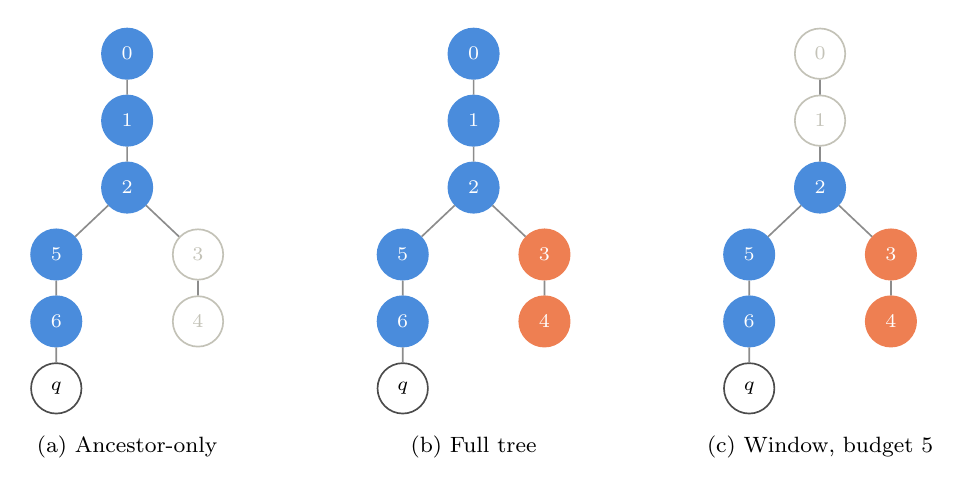
\begin{tikzpicture}[
  msg/.style={circle, draw, minimum size=6.4mm, inner sep=0pt, font=\scriptsize, line width=0.6pt},
  on/.style={msg, fill=ancblue!85, draw=ancblue!85, text=white},
  sib/.style={msg, fill=sibor!85, draw=sibor!85, text=white},
  off/.style={msg, draw=offgray, text=offgray, fill=white},
  q/.style={msg, draw=black!70, fill=white},
  edge/.style={-, line width=0.6pt, color=black!45},
  lab/.style={font=\footnotesize, align=center}]
\newcommand{\tree}[8]{%
  \begin{scope}[shift={(#1,0)}]
    \node[#2] (r) at (0,0) {0}; \node[#3] (m) at (0,-0.85) {1}; \node[#4] (f) at (0,-1.7) {2};
    \node[#5] (s1) at (0.9,-2.55) {3}; \node[#6] (s2) at (0.9,-3.4) {4};
    \node[#7] (a1) at (-0.9,-2.55) {5}; \node[#8] (a) at (-0.9,-3.4) {6}; \node[q] (qq) at (-0.9,-4.25) {$q$};
    \draw[edge] (r)--(m) (m)--(f) (f)--(s1) (s1)--(s2) (f)--(a1) (a1)--(a) (a)--(qq);
  \end{scope}}
\tree{0}{on}{on}{on}{off}{off}{on}{on}
\tree{4.4}{on}{on}{on}{sib}{sib}{on}{on}
\tree{8.8}{off}{off}{on}{sib}{sib}{on}{on}
\node[lab] at (0,-5.0) {(a) Ancestor-only};
\node[lab] at (4.4,-5.0) {(b) Full tree};
\node[lab] at (8.8,-5.0) {(c) Window, budget 5};
\end{tikzpicture}
\end{center}

How to read it:
\begin{itemize}
\item Messages 0, 1, 2 come first. At message 2 the conversation branches.
\item Messages 3 and 4 are a side exploration (the orange sibling branch).
\item The user then returns to message 2 and continues the main line with messages 5 and 6. Message 6 is the \term{ask node}: the question $q$ is asked as its reply.
\item Blue means ``on the active path and sent''. Orange means ``sibling content and sent''. Grey outline means ``not sent''.
\end{itemize}

What each rule sends, if every message is the same size:
\begin{itemize}
\item Ancestor-only sends 0, 1, 2, 5, 6. That is five messages, so the budget for the window is 5.
\item Full tree sends all seven, in time order 0, 1, 2, 3, 4, 5, 6.
\item The window walks back from the newest: 6, 5, 4, 3, 2. Five messages fill the budget, so it stops. Messages 0 and 1 are dropped, even though they are on the active path, and the sibling messages 3 and 4 are sent instead.
\end{itemize}

\begin{plain}
The window is the same size as ancestor-only, but it spends part of its space on the abandoned branch and pays for it by forgetting the start of the conversation. If the decision you are asking about was made at the start, the window has thrown it away.
\end{plain}

\section{The running example, message by message}

Now the real scenario. The developer chooses LRU in the very first message (m1). After four messages, three sibling branches explore LFU, ARC and FIFO (m5 to m22). Then the developer returns to the main line (m23 to m26) and asks the question. Each message's token weight $w$ is from the reference tokenizer.

\begin{center}
\small
\begin{tabular}{@{}llllrl@{}}
\toprule
Message & Time $t$ & Branch & Role & $w$ & Content (start) \\
\midrule
m1 & 0 & active & user & 39 & ``\dots let's go with LRU.'' \\
m2 & 1 & active & assistant & 67 & ``LRU is a reasonable fit \dots'' \\
m3 & 2 & active & user & 31 & negative lookups? \\
m4 & 3 & active & assistant & 69 & (answer; the fork point) \\
m5--m10 & 4--9 & s1 & both & 273 & ``What if we used LFU \dots'' \\
m11--m16 & 10--15 & s2 & both & 320 & ``Would ARC eviction \dots'' \\
m17--m22 & 16--21 & s3 & both & 326 & ``What if we used FIFO \dots'' \\
m23 & 22 & active & user & 45 & measuring the cache \\
m24 & 23 & active & assistant & 57 & (answer) \\
m25 & 24 & active & user & 42 & entry lifetime \\
m26 & 25 & active & assistant & 67 & (answer; the ask node) \\
\midrule
\multicolumn{4}{@{}l}{Total of all 26 messages} & 1{,}336 & \\
\multicolumn{4}{@{}l}{Active path (m1--m4, m23--m26)} & 417 & \\
\multicolumn{4}{@{}l}{Siblings (m5--m22)} & 919 & \\
\bottomrule
\end{tabular}
\end{center}

\begin{example}
\textbf{Ancestor-only} sends m1, m2, m3, m4, m23, m24, m25, m26: 417 tokens.

\textbf{Full tree} sends all 26 messages: 1,336 tokens.

\textbf{Window} has a budget of 417. Walking back from the newest:
m26 (67, running total 67), m25 (42, 109), m24 (57, 166), m23 (45, 211), m22 (73, 284), m21 (40, 324), m20 (77, 401). The next one, m19, is 44 tokens; $401 + 44 = 445 > 417$, so the window stops. It sends m20 to m26: 401 tokens, which is $401/417 = 96.2\%$ of the budget.

The window kept the last four active messages and three messages from the FIFO branch. It dropped m1, the message where LRU was chosen.
\end{example}

\section{What the models said}

Here is what GPT-6.2 Sol answered to ``which eviction policy did we choose for the product cache? Give me the config line'' under each rule.

\begin{example}[: GPT-6.2 Sol]
\textbf{Ancestor-only:} ``We chose \textbf{LRU} (least recently used).'' followed by \texttt{evictionPolicy: LRU}. Correct, faithful, complete.

\textbf{Full tree:} ``We chose \textbf{LRU}. Using \texttt{eviction\_policy} as the config key:'' followed by \texttt{eviction\_policy: lru}. Correct. The siblings were in front of it, but it was not misled.

\textbf{Window:} ``We didn't choose an eviction policy earlier. I'd use \textbf{LRU} for the first version.'' The decision was no longer in its prompt, so it said no decision had been made, then happened to recommend LRU anyway.
\end{example}

The window answer is a good warning about measurement. It contains the word ``LRU'', so a simple check would mark it correct. But it is right for the wrong reason: it says the decision was never made. The quality judge caught this and gave it 2 out of 5 for faithfulness. Chapter 7 explains how the scoring handles cases like this.

\begin{ask}
\textbf{``Isn't the window just a strawman? Nobody would build it that way.''}\par
Sliding windows are a standard, widely used way to keep chat prompts short, and the paper's related work cites them. The window here is the most common form (newest messages first, whole messages only), and it was given exactly the same token budget as ancestor-only, which is the fairest possible comparison. Its failure is not a quirk of implementation; Propositions 5 and 6 prove it must drop the oldest active messages whenever siblings take up space.
\end{ask}

\chapter{The formulas, one symbol at a time}

This is the chapter to read slowly. Section III of the paper uses mathematical notation to say precisely what the three rules do, and then proves six short facts (``propositions'') about them. None of the mathematics is hard once each symbol is clear. Each proposition below gets four treatments: the paper's wording, the meaning in plain words, a check with the running example's real numbers, and a walk through the proof.

\section{A notation primer}

\begin{center}
\small
\begin{tabularx}{\textwidth}{@{}lX@{}}
\toprule
Symbol & How to read it and what it means \\
\midrule
$\{a, b, c\}$ & ``the set containing $a$, $b$ and $c$''. A \term{set} is a collection with no order and no repeats. \\
$x \in U$ & ``$x$ is in $U$''; $x$ is one of the members of set $U$. \\
$U \subseteq V$ & ``$U$ is a subset of $V$''; every member of $U$ is also in $V$. \\
$U \cap V$ & ``$U$ intersect $V$''; the members in both. \\
$U \cup V$ & ``$U$ union $V$''; the members in either. \\
$U \,\dot\cup\, V$ & a \term{disjoint union}: a union where $U$ and $V$ share no members. \\
$V \setminus U$ & ``$V$ minus $U$''; the members of $V$ that are not in $U$. \\
$\varnothing$ & the empty set, with no members. \\
$|U|$ & the number of members of $U$. \\
$\sum_{u \in U} w(u)$ & ``the sum over every $u$ in $U$ of $w(u)$''; add up $w$ for each member. \\
$f\colon X \to Y$ & a \term{function} $f$ that takes something from $X$ and gives something in $Y$. \\
$\Pr(M \mid c)$ & ``the probability of $M$ given $c$''; how often $M$ happens when $c$ holds. \\
$\mathbf{1}[\ldots]$ & an \term{indicator}: 1 if the statement in brackets is true, 0 if it is false. \\
$\Theta(n^2)$, $O(n)$ & growth rates. $O(n)$ means ``grows no faster than proportionally to $n$''. $\Theta(n^2)$ means ``grows like $n^2$, both at least and at most up to a constant''. \\
$\lfloor x \rfloor$ & the \term{floor} of $x$: round down to a whole number. $\lfloor 4/2 \rfloor = 2$, $\lfloor 5/2 \rfloor = 2$. \\
$\square$ or $\blacksquare$ & end of a proof. \\
\bottomrule
\end{tabularx}
\end{center}

\section{The setting}

\begin{paper}
A session is a rooted tree $T=(V,E)$ of messages with root $r$ and parent map $p$. A logical clock $\tau$ is injective and increases along every edge, and each message has a token weight $w(v)>0$ under a fixed reference tokenizer; for $U\subseteq V$, $w(U)=\sum_{u\in U}w(u)$.
\end{paper}

Taking the sentence apart:

\begin{itemize}
\item \textbf{Session.} One conversation.
\item \textbf{$T = (V, E)$.} A tree is described by two sets. $V$ (``vertices'') is the set of messages. $E$ (``edges'') is the set of parent--child links. In the running example, $V = \{m1, m2, \dots, m26\}$, so $|V| = 26$.
\item \textbf{Root $r$.} The first message. In the example, $r = m1$.
\item \textbf{Parent map $p$.} A function: $p(v)$ is the parent of message $v$. In the example, $p(m2) = m1$, $p(m5) = m4$, and $p(m23) = m4$. The root has no parent.
\item \textbf{Logical clock $\tau$.} A function giving each message a whole number for when it was written: $\tau(m1) = 0$, $\tau(m2) = 1$, and so on up to $\tau(m26) = 25$. (The Greek letter $\tau$ is ``tau''.)
\item \textbf{Injective.} No two messages share a time. Every message has its own number.
\item \textbf{Increases along every edge.} A reply is always written after the message it replies to: $\tau(p(v)) < \tau(v)$.
\item \textbf{Token weight $w(v) > 0$.} The number of reference tokens in message $v$. Every message has at least one token.
\item \textbf{$w(U)$.} The total weight of a set of messages: add up their weights.
\end{itemize}

\begin{example}
$w(m1) = 39$, $w(m2) = 67$. For the set $U = \{m1, m2\}$, $w(U) = 39 + 67 = 106$. For the whole tree, $w(V) = 1{,}336$.
\end{example}

\begin{paper}
A question $q$ is asked as a child of an ask node $a$, later than every message. The active path is $A(a)=\{a,p(a),\dots,r\}$ and the sibling content is $S(a)=V\setminus A(a)$.
\end{paper}

\begin{itemize}
\item \textbf{Ask node $a$.} The last message before the question. In the example, $a = m26$.
\item \textbf{$A(a)$, the active path.} The ask node, its parent, its parent's parent, and so on up to the root. In the example:
\[A(m26) = \{m26, m25, m24, m23, m4, m3, m2, m1\}.\]
Note how the path jumps from m23 straight to m4: m23's parent is m4, because the main line resumed from m4 after the side branches.
\item \textbf{$S(a) = V \setminus A(a)$, the sibling content.} Every message that is not on the active path. In the example, $S(m26) = \{m5, \dots, m22\}$, the 18 messages of the three side branches.
\end{itemize}

\begin{example}
$w(A(a)) = 39+67+31+69+45+57+42+67 = 417$ and $w(S(a)) = 1{,}336 - 417 = 919$.
\end{example}

\section{The three rules as formulas}

\begin{paper}
Ancestor-only: $C_\anc=A(a)$, ordered root to node. Full tree: $C_\full=V$, ordered by $\tau$. Sliding window: $C_\win$ is the longest run of newest messages whose total weight is at most $B=w(A(a))$, never splitting a message.
\end{paper}

$C$ stands for ``context'': the set of messages a rule sends. The subscript names the rule. $B$ is the window's \term{budget}, defined as the weight of the active path.

\begin{example}
$C_\anc = A(a)$, weight 417. $C_\full = V$, weight 1,336. $B = 417$, and $C_\win = \{m20, \dots, m26\}$, weight 401 (worked out in Chapter 3).
\end{example}

\section{Proposition 1: token efficiency}

\begin{paper}
$C_\anc\subseteq C_\full$, and the token efficiency equals the siblings' share of the tree: $E=1-\dfrac{w(C_\anc)}{w(C_\full)}=\dfrac{w(S(a))}{w(V)}$.
\end{paper}

\begin{plain}
Two claims. First, everything ancestor-only sends, the full tree also sends, so ancestor-only can never be bigger. Second, the fraction of tokens ancestor-only saves is exactly the fraction of the conversation taken up by abandoned branches. If side branches make up 70\% of the conversation, ancestor-only saves 70\%.
\end{plain}

\textbf{What $E$ is.} $E$ is \term{token efficiency}: one minus the ratio of the two sizes. If ancestor-only were the same size as the full tree, the ratio is 1 and $E = 0$ (no saving). If ancestor-only were tiny, $E$ is close to 1 (almost everything saved).

\begin{example}
$E = 1 - 417/1{,}336 = 1 - 0.312 = 0.688$, a saving of 68.8\%.\par
$w(S(a))/w(V) = 919/1{,}336 = 0.688$. The two numbers agree, as the proposition says.
\end{example}

\textbf{The proof, step by step.}
\begin{enumerate}
\item Every message on the active path is a message of the tree, so $A(a) \subseteq V$, which means $C_\anc \subseteq C_\full$.
\item Weights are positive, so a subset can never weigh more: $w(C_\anc) \le w(C_\full)$.
\item Every message is either on the active path or not, never both. So $V$ splits into two non-overlapping parts, $V = A(a) \,\dot\cup\, S(a)$, and the weights add: $w(V) = w(A(a)) + w(S(a))$.
\item Divide both sides by $w(V)$: $1 = \frac{w(A(a))}{w(V)} + \frac{w(S(a))}{w(V)}$. Rearranged, $1 - \frac{w(A(a))}{w(V)} = \frac{w(S(a))}{w(V)}$, which is the formula.
\end{enumerate}

\begin{plain}
The proof is really just ``the whole is the sum of its two parts''. It is short because the claim is simple. Its value is that it turns ``how much does ancestor-only save?'' from an experimental question into arithmetic you can do from the tree alone, before running any model.
\end{plain}

\begin{ask}
\textbf{``If it's just arithmetic, why measure it?''}\par
To check the implementation, not the mathematics. The measured savings matched the formula in all 720 scenarios to within $1.1 \times 10^{-16}$ (the rounding limit of a computer). That shows the code builds the prompts exactly as defined. It also gives a planning tool: Traceback can predict its savings from the shape of a conversation.
\end{ask}

\section{Proposition 2: growth over a session}

\begin{paper}
If a session grows one message at a time, each step re-sends its context, weights lie in $[w_{\min},w_{\max}]$ and the answered depth is at most $D$, the cumulative full-tree cost is at least $w_{\min}n(n+1)/2=\Theta(n^2)$, while the cumulative ancestor-only cost is at most $w_{\max}n(D+1)=O(nD)$.
\end{paper}

\begin{plain}
In a real chat, the prompt is re-sent on every turn. With the full tree, turn 1 sends 1 message, turn 2 sends 2, turn 3 sends 3, and so on. The total over a long conversation grows with the \emph{square} of its length. With ancestor-only, each turn sends only one path, whose length is limited by how deep the conversation goes. If depth stays bounded, the total grows only in a straight line.
\end{plain}

\textbf{The pieces.}
\begin{itemize}
\item $n$ is the number of messages so far. $V_t$ is the tree after $t$ messages, so $|V_t| = t$.
\item $w_{\min}$ and $w_{\max}$ are the smallest and largest message weights.
\item $D$ is the deepest depth that ever gets answered.
\item $1 + 2 + \dots + n = n(n+1)/2$, a classic formula (try $n = 4$: $1+2+3+4 = 10 = 4 \times 5 / 2$).
\end{itemize}

\textbf{The proof.} At step $t$ the full tree has $t$ messages, each at least $w_{\min}$ tokens, so it costs at least $t \cdot w_{\min}$. Summing over $t = 1, \dots, n$ gives at least $w_{\min}(1 + 2 + \dots + n) = w_{\min} n(n+1)/2$. A path at depth $d_t$ has $d_t + 1$ messages, each at most $w_{\max}$, so it costs at most $(d_t + 1)w_{\max} \le (D+1)w_{\max}$; summing $n$ of these gives at most $w_{\max} n (D+1)$.

\begin{example}
Suppose every message is 50 tokens and the conversation reaches 100 messages, with depth never above 20. Full tree, total over the session: at least $50 \times 100 \times 101 / 2 = 252{,}500$ tokens. Ancestor-only: at most $50 \times 100 \times 21 = 105{,}000$. At 1,000 messages the full tree passes 25 million tokens, while ancestor-only stays at about 1 million.
\end{example}

\begin{why}
This proposition is not tested in the experiment, which asks one question per scenario. It is there to explain why the token saving matters in practice: over a long session the gap is not a constant percentage but grows.
\end{why}

\section{Proposition 3: no sibling facts under ancestor-only}

\begin{paper}
If every message containing a fact $f$ lies in $S(a)$ and $q$ does not contain $f$, then $f$ is absent from the ancestor-only prompt.
\end{paper}

\begin{plain}
If a piece of information only appears in abandoned branches (and not in the question), then ancestor-only cannot show it to the model, because ancestor-only only sends the active path and the question.
\end{plain}

\textbf{The proof.} The ancestor-only prompt is the text of the messages in $A(a)$ followed by $q$. The active path and the siblings share no messages ($A(a) \cap S(a) = \varnothing$). Every message containing $f$ is in $S(a)$, so none is in $A(a)$; and $q$ does not contain $f$. So $f$ is nowhere in the prompt.

\begin{example}
The canary \texttt{orbit\_y5y} appears only in m6, in branch s1. m6 is not on the active path, so the ancestor-only prompt never contains it. Across all 2,598 ancestor-only answers in the full run (including repeats), not one contained a canary.
\end{example}

\begin{plain}
The consequence is important for measurement. Under ancestor-only, a model can only produce a sibling-only fact by \emph{chance}. For a random canary, chance is essentially zero. For a forced-choice value such as ``LRU'', chance is not zero: a model might guess a common option. That is why the paper measures leakage against what ancestor-only produces, not against zero.
\end{plain}

\section{Proposition 4: exposure times uptake}

\begin{paper}
Let $X_c(f)$ indicate that $f$ is in the prompt of rule $c$, $\pi_f$ the rate of mentioning $f$ without seeing it, and $u_c(f)$ the rate when exposed. $X_c(f)$ is a function of $(T,\tau,w,a)$ alone, and for a sibling-only fact $\Pr(M\mid c)-\Pr(M\mid\anc)=X_c(f)\,\bigl(u_c(f)-\pi_f\bigr)$.
\end{paper}

\textbf{The symbols.}
\begin{itemize}
\item $c$ is one of the rules: anc, full or win.
\item $M$ is the event ``the model's answer mentions $f$''.
\item $X_c(f)$ is the \term{exposure}: 1 if $f$ is in rule $c$'s prompt, 0 if not.
\item $\pi_f$ (Greek ``pi'') is the \term{chance rate}: how often a model mentions $f$ without ever seeing it.
\item $u_c(f)$ is the \term{uptake}: how often it mentions $f$ when $f$ is in the prompt.
\item The left side is the \term{excess} mention rate of rule $c$ over ancestor-only.
\end{itemize}

\begin{plain}
Leakage can be split into two parts. \emph{Exposure}: was the sibling fact in the prompt at all? That depends only on the tree and the rule, so it can be computed without running any model. \emph{Uptake}: when the fact was there, did the model use it? That needs the model. If the fact was not exposed, a rule cannot leak it beyond chance; if it was, the extra leakage is uptake minus chance.
\end{plain}

\textbf{The proof.} By Proposition 3, the ancestor-only rate is just the chance rate: $\Pr(M \mid \anc) = \pi_f$. Under rule $c$, there are two cases. If $X_c(f) = 0$, the fact is not in the prompt, so the rate is again $\pi_f$ and the difference is $0 = 0 \cdot (u_c - \pi_f)$. If $X_c(f) = 1$, the rate is $u_c(f)$ and the difference is $u_c(f) - \pi_f = 1 \cdot (u_c - \pi_f)$. Both cases match the formula.

\begin{example}
In the running example the window prompt (m20 to m26) contains no canary and no conflicting value: the planted items sit in the first exchange of each branch (m5--m6, m11--m12, m17--m18), and the window only reached m20. So $X_\win = 0$ for every planted item, and the window could not leak them. The full tree contains all of them ($X_\full = 1$); Gemini's full-tree answer used one, \texttt{orbit\_q8y}, in its config line.
\end{example}

\begin{why}
This is why the experiment logs exposure for every single call, and why window leakage is analysed among exposed calls (``uptake''). In your dataset only 18\% of canaries landed in a window prompt, because they were planted early in each branch and the window keeps late messages. You chose to keep that design and analyse leakage conditional on exposure, rather than move the planted facts.
\end{why}

\section{Proposition 5: which messages the window keeps}

\begin{paper}
A message $m$ is in $C_\win$ if and only if $\sum_{u:\,\tau(u)\ge\tau(m)}w(u)\le B$. Hence, whenever $S(a)\neq\varnothing$, the root is never in the window, since that sum for $r$ is $w(V)=B+w(S(a))>B$.
\end{paper}

\textbf{Reading the condition.} $\sum_{u:\,\tau(u)\ge\tau(m)} w(u)$ means ``add up the weights of $m$ and every message written after it''. Call this $m$'s \term{suffix sum}. The proposition says: $m$ is in the window exactly when its suffix sum fits in the budget.

\begin{plain}
The window takes the newest messages first. A message gets in only if it and everything newer than it fit in the budget together. The very first message has everything newer than it, which is the whole conversation. If there are any side branches, the whole conversation is bigger than the active path, so the first message can never fit.
\end{plain}

\begin{example}
Budget $B = 417$.\par
m23: suffix sum $= 45 + 57 + 42 + 67 = 211 \le 417$, so m23 is in.\par
m20: suffix sum $= 77 + 40 + 73 + 211 = 401 \le 417$, so m20 is in.\par
m19: suffix sum $= 44 + 401 = 445 > 417$, so m19 is out.\par
m1 (the root): suffix sum $= w(V) = 1{,}336 > 417$, so m1 is out. The decision ``let's go with LRU'' is gone.
\end{example}

\textbf{The proof.} The window adds messages newest-first and stops at the first one that does not fit. Because every weight is positive, each running total is bigger than the one before. So the messages that fit form an unbroken run starting from the newest, and a message is included exactly when the running total up to and including it, which is its suffix sum, is at most $B$. For the root, the suffix sum is $w(V)$; by Proposition 1's split, $w(V) = w(A(a)) + w(S(a)) = B + w(S(a))$, which is more than $B$ whenever there is at least one sibling message.

\begin{example}
Across all 720 scenarios, this test predicted correctly whether the required fact was in the window prompt every time (720 of 720). In the 360 scenarios where the fact sat at the root, it was in the window 0 times.
\end{example}

\section{Proposition 6: one-for-one displacement}

\begin{paper}
If $\sigma=w(C_\win\cap S(a))$ sibling tokens enter the window, at least $\sigma$ active-path tokens leave it, and the active messages lost are always the oldest. If all siblings are newer than $a$, the message $m$ holding the required fact survives if and only if $w(S(a))\le w(\{u\in A(a):\tau(u)<\tau(m)\})$.
\end{paper}

\textbf{The symbols.} $\sigma$ (Greek ``sigma'') is the number of sibling tokens inside the window. $C_\win \cap S(a)$ is ``the window's messages that are sibling messages''.

\begin{plain}
Three claims. (1) The window has the same budget as the active path, so every sibling token that gets in pushes out at least one active-path token. (2) The active messages pushed out are always the earliest ones. (3) When the siblings were all explored after the active path (``late'' siblings), a fact survives only if the siblings are no bigger than everything on the active path written before that fact.
\end{plain}

\begin{example}
Window: m20, m21, m22 are sibling messages, so $\sigma = 77 + 40 + 73 = 190$. The active messages in the window are m23 to m26, weight 211. Active tokens lost: $417 - 211 = 206$, which is at least $\sigma = 190$, as claimed. The lost messages are m1, m2, m3, m4, the oldest four.
\end{example}

\textbf{The proof.} (1) The window's weight is its active part plus its sibling part, and that cannot exceed the budget: $w(C_\win \cap A(a)) + \sigma \le B = w(A(a))$. Rearranging, $w(A(a)) - w(C_\win \cap A(a)) \ge \sigma$; the left side is exactly the active tokens left out. (2) If an active message is kept, a newer active message has a smaller suffix sum, so by Proposition 5 it is kept too; the kept active messages are therefore always the newest ones. (3) With late siblings, everything newer than $m$ is the siblings plus the active messages from $m$ onward. Put that into Proposition 5's test with $B = w(A(a))$ and cancel the active part.

\begin{example}
For the 360 late-sibling scenarios, the survival condition in (3) was correct every time (360 of 360). It explains why the required fact survived in only 16.1\% of the late/current-turn cases: in most of them the siblings were heavier than the active messages before the fact.
\end{example}

\section{How the formulas connect to the results}

\begin{center}
\small
\begin{tabularx}{\textwidth}{@{}lXl@{}}
\toprule
Proposition & What it predicts & What happened \\
\midrule
1 & Savings equal the siblings' share & Exact in 720/720 \\
3 & No sibling canary under ancestor-only & 0 of 2,598 answers \\
4 & Leakage needs exposure & Window leaks only where exposed \\
5 & Root facts never in the window & 0 of 360 root scenarios \\
5 & Exact list of messages the window keeps & 720/720 \\
6 & Late siblings: survival condition & 360/360 \\
\bottomrule
\end{tabularx}
\end{center}

\begin{ask}
\textbf{``Your propositions are trivial. Where is the contribution?''}\par
They are meant to be simple; your advisor asked for minimal theory. Their contribution is that they turn the results from observations into consequences. Without them, ``the window got half the answers wrong'' is a finding that might depend on the models. With them, it follows from how a recency window works on a branched conversation: whenever side branches take up space, the earliest active messages must be dropped. The models only decide what happens next, once the fact is gone.
\end{ask}

\chapter{How the test conversations were built}

The paper's Methodology section, part A, describes the 720 scenarios. This chapter explains every choice behind them.

\section{Why synthetic conversations}

\begin{why}
Real chat logs would be more natural, but you would not know, for any given answer, which facts lived only in an abandoned branch, or what the right answer was. Synthetic conversations let you plant every fact on purpose, so the correct answer and every possible leak are known exactly before a model sees anything. The price is realism, which the paper lists as a limitation.
\end{why}

\section{The six topics}

Every scenario is a programming conversation in one of six domains, with a question whose answer is one of seven options:

\begin{center}
\small
\begin{tabularx}{\textwidth}{@{}lXX@{}}
\toprule
Domain & The decision & The seven options \\
\midrule
db & primary key type for the users table & uuid, bigserial, ulid, ksuid, cuid2, snowflake, nanoid \\
http & HTTP client library for a Node service & undici, axios, ky, superagent, ofetch, wretch, phin \\
cache & eviction policy for a product cache & LRU, LFU, FIFO, ARC, SLRU, 2Q, MRU \\
flaky & root cause of a flaky checkout test & timezone, locale, unseeded-random, shared-fixture, port-collision, stale-snapshot, mock-leak \\
queue & message broker for order events & RabbitMQ, Kafka, NATS, SQS, BullMQ, Pulsar, ZeroMQ \\
auth & password hashing algorithm & argon2id, bcrypt, scrypt, pbkdf2, yescrypt, balloon, sha512crypt \\
\bottomrule
\end{tabularx}
\end{center}

\begin{why}
Six domains, so that a result cannot be blamed on one topic (your brief asked for at least six). Each answer is a \term{forced-choice} value: one specific word that is easy to check automatically. Seven options per domain, because a scenario can have up to five conflicting siblings, and each needs its own wrong option, plus the correct one.
\end{why}

\section{The five things that vary}

\begin{paper}
Table I lists the controlled variables; with five instances per cell the benchmark has 720 scenarios and 19,680 messages.
\end{paper}

A \term{controlled variable} is something you deliberately set to different levels to see its effect. There are five:

\begin{enumerate}
\item \textbf{Active-path depth: 2, 4 or 8 exchanges.} How long the main line is before the question. Longer paths mean bigger ancestor-only prompts and bigger window budgets.
\item \textbf{Number of sibling branches: 1, 3 or 5}, each 3 exchanges long. More siblings mean more abandoned content.
\item \textbf{Sibling type: consistent, conflicting, irrelevant or misleading.} What the abandoned branch contains (next section).
\item \textbf{Sibling recency: early or late.} Whether the side branches were explored before the main line continued (early) or after the main line had finished (late).
\item \textbf{Position of the required fact: near the root or near the current turn.} Whether the decision was made at the start (exchange 1) or at the end (the last exchange) of the active path.
\end{enumerate}

\begin{example}
Every combination is a \term{cell}: $3 \times 3 \times 4 \times 2 \times 2 = 144$ cells. Five scenarios per cell gives $144 \times 5 = 720$. Each domain appears 120 times, each sibling type 180 times, and each depth and sibling count 240 times. The running example sits in the cell ``depth 4, 3 siblings, conflicting, early, root''.
\end{example}

\section{The four sibling types}

\begin{plain}
\textbf{Consistent:} the side branch agrees with the main decision and adds an extra true detail. \textbf{Conflicting:} the side branch picks a different option. \textbf{Misleading:} the side branch states something plausible but false. \textbf{Irrelevant:} the side branch is about something unrelated.
\end{plain}

Real examples from your dataset:

\begin{example}[: consistent sibling]
Main decision: cuid2 keys. Side branch: ``If we stick with cuid2 keys, how should we generate them?'' Reply: ``\dots name the column \texttt{zr\_9fg} so it is clear it is the external id.'' The detail \texttt{zr\_9fg} is true to the plan but was never said on the active path.
\end{example}

\begin{example}[: misleading sibling]
Main decision: bigserial keys. Side branch: ``I read that since Postgres 7.32.32, bigserial keys have to be declared through a special domain type or inserts get slow. Is that right?'' Reply: ``Yes, that matches the release notes \dots'' This is false, and the made-up version number 7.32.32 is its canary.
\end{example}

\begin{example}[: irrelevant sibling]
``Off topic: I need a name for the team's internal wiki space and I'm thinking of \texttt{kq\_8wr}.'' Nothing to do with caching; \texttt{kq\_8wr} is the canary.
\end{example}

\begin{example}[: conflicting sibling]
Main decision: LRU. Side branch: ``What if we used LFU for the product cache eviction instead?'' Reply: ``LFU could work too. I'd put the policy behind a setting called \texttt{orbit\_y5y} \dots'' Both LFU (a real wrong option) and \texttt{orbit\_y5y} (the canary) are leak markers.
\end{example}

\begin{why}
The four types come straight from your thesis outline. The earlier study saw its biggest gains when tangents were ``conceptually distant or conflicting'', but did not vary this on purpose. Making type a controlled variable turns that observation into a test. The consistent type exists specifically to measure the possible \emph{price} of ancestor-only: a consistent sibling holds true, useful information that ancestor-only throws away.
\end{why}

\section{Canaries}

Every sibling-only detail carries a canary: a random identifier (like \texttt{orbit\_y5y}), a 4-digit number, a hex colour (like \texttt{\#4A7F2C}) or a version number. The generator makes sure each canary appears exactly once, only in its own branch.

\begin{plain}
If an answer contains \texttt{orbit\_y5y}, the model read it in the side branch. Nobody could guess that string. This turns ``did the model use the abandoned branch?'' into a simple text search, at least as a first step.
\end{plain}

\section{Where siblings branch off, and when}

\begin{why}
Siblings branch off the active path at exchange $\lfloor d/2 \rfloor$, the middle of the path (exchange 2 for depth 4). This is what makes ``fact position'' meaningful: a root-side fact was stated \emph{before} the branch point, so the siblings share it in their own history; a current-turn fact was stated \emph{after}, so the siblings never saw it. You chose this default when Phase 1 was built; the alternatives were branching from the root or from the last message.
\end{why}

Recency is set with the logical clock:
\begin{itemize}
\item \textbf{Early:} active exchanges up to the branch point, then all the siblings, then the rest of the active path. The siblings sit in the middle of the timeline.
\item \textbf{Late:} the whole active path first, then all the siblings. The siblings are the newest messages.
\end{itemize}

In both cases the question is asked after everything else, at time $\max(t) + 1$, as if the user explores, then comes back to the main line to ask. That is why the full tree contains late siblings too.

\section{The required fact and the question}

The correct option is stated on the active path in exactly one exchange: exchange 1 (root) or the last exchange (current turn). The final question always asks for that value and a line of code or config, so an answer must name it. The question never contains any of the options.

\section{Filling text and padding}

The planted sentences come from templates. To make conversations a realistic length, each message is padded with neutral sentences (``We can revisit this once we have real traffic numbers.'') until it reaches a target token length. User messages are 22 to 52 tokens and assistant messages 45 to 90. Off-topic branches get off-topic padding.

\begin{ask}
\textbf{``The padding makes the conversations repetitive. Doesn't that hurt realism?''}\par
Yes, and it is listed as a limitation. It was chosen so that every planted fact stays exactly where it was placed and the dataset is fully reproducible from a seed. An LLM rewrite of the filler was considered and left out to avoid changing planted facts by accident. The padding is the same in every condition, so it cannot explain differences between conditions.
\end{ask}

\section{Checking every scenario: the validator}

Before the dataset was frozen, a validator checked each of the 720 scenarios and would have refused to write the file if any check failed:
\begin{itemize}
\item the tree is well formed, with one root and alternating roles;
\item each reply is written after its parent;
\item the active path is exactly the messages marked ``active'';
\item siblings branch at the right point, with the right size;
\item the timestamps match the recency level;
\item each canary appears exactly once, in its own branch;
\item no sibling value appears anywhere on the active path or in the question;
\item the required fact sits at the stated position and nowhere else on the path;
\item every message is within the length band.
\end{itemize}
Tests also deliberately corrupted scenarios (for example, copying a canary into the active path) and confirmed the validator caught each one.

\section{Freezing the dataset}

\begin{plain}
Before any model saw the full dataset, the file was fingerprinted (sha256 \texttt{4c3e5380\dots c37d}), the fingerprint was saved, and the exact code version was labelled with the git tag \texttt{thesis-freeze-v1}. Anyone can regenerate the file from the seed and get the identical fingerprint. This shows the test was not adjusted after seeing results.
\end{plain}

\section{Loading into Traceback}

The scenarios were loaded into a separate experiment database (a Neon project created only for this), using Traceback's own database schema and code. Each scenario became one normal Traceback session, with message ids like \texttt{exp-<scenario>-m1}, and \texttt{created\_at} set from the logical clock (one tick per minute). A safety guard refused to run any script against the production database. Loading was checked row by row and was repeatable: loading twice produced an identical database fingerprint.

\chapter{Running the models}

\section{Which models and why}

\begin{center}
\small
\begin{tabularx}{\textwidth}{@{}llX@{}}
\toprule
Role & Model & Why this one \\
\midrule
Frontier & Gemini 4 Argon & Google's flagship; accepts temperature 0 and a seed, so it is as repeatable as possible. Cheaper than OpenAI's flagship. \\
Mid-size & GPT-6.2 Sol & OpenAI's model below its flagship; the most widely used family. Cannot be set to temperature 0 through OpenRouter. \\
Open weights & Mistral Large 4 & Its weights are public; served only by Mistral, so there is no variation between hosting providers. \\
Judge & Claude Opus 5.5 & A strong model from a family not being tested, so it is not grading its own family. \\
\bottomrule
\end{tabularx}
\end{center}

\begin{why}
Three families (Google, OpenAI, Mistral) so the result is not about one company's models. A judge from a fourth family (Anthropic) avoids a model grading answers from its own family, which is a known source of bias.
\end{why}

\section{How each call was made}

\begin{itemize}
\item Every call went through OpenRouter, \textbf{locked to one provider} with fallbacks off. A log line records which provider actually answered; every call used the intended one.
\item The \textbf{same system prompt} for every model and condition.
\item \textbf{Lowest reasoning setting} and a \textbf{1,024-token output cap}.
\item \textbf{Temperature 0} where the API allowed it.
\item No tools and no web search: the model sees only the prompt.
\end{itemize}

\section{How many calls}

Each model answered all 720 scenarios under all 3 conditions: 2,160 calls. A random 10\% of scenarios (73 of them) were run three times instead of once, to measure how much answers change between runs. That adds $73 \times 3 \times 2 = 438$ calls, for $2{,}160 + 438 = 2{,}598$ per model and 7,794 in total.

\begin{plain}
The ``first run'' of each scenario is the one used in the main analysis (6,479 answered calls across the three models). The two extra runs exist only to check repeatability.
\end{plain}

\section{The pilot}

Before the full run, 20 scenarios were run on Mistral (60 calls, \$0.08). The pilot checked that canaries could be detected, that ancestor-only produced no false alarms, that window sizes were close to their budget, and that cost matched the estimate (it was 1.06 times the estimate). It also showed that simple string matching over-counts leaks, which is why a judge was added for leaks.

\section{Deviation D1: Mistral answers that were cut off}

\begin{plain}
On 107 of 2,598 Mistral calls, the model spent almost its whole 1,024-token allowance thinking and ran out before finishing its answer; 62 of those produced no answer at all. These 107 calls were re-sent with exactly the same prompt and a larger allowance of 4,096 tokens. 106 then finished normally. One still did not, and counts as ``no answer''.
\end{plain}

\begin{why}
The alternative was to count the 107 as failures. They were spread across all three conditions (4.6\% ancestor, 3.9\% full tree, 3.8\% window), slightly more often under ancestor-only, so leaving them would have wrongly made ancestor-only look worse. Raising the cap only matters for calls that hit it: every other call finished well under 1,024 tokens, so giving them more room would not have changed them. The replay used the exact logged prompt, byte for byte. This is recorded as deviation D1 in \texttt{DEVIATIONS.md}, with the rule that the replayed answers replace the originals.
\end{why}

A side observation: 59 of the 107 replays finished in under 1,024 tokens even though the identical prompt had not the first time. So Mistral is not fully deterministic even at temperature 0 with a fixed seed. The repeat runs measure how much this matters (Chapter 9).

\section{Cost}

\begin{center}
\small
\begin{tabular}{@{}lr@{}}
\toprule
Item & Cost (US\$) \\
\midrule
Gemini 4 Argon (2,598 calls) & 7.74 \\
GPT-6.2 Sol (2,598 calls) & 5.96 \\
Mistral Large 4 (2,598 calls + 107 replays) & 3.79 \\
Pilot & 0.08 \\
Judge (9,257 judgments + pilots) & 68.55 \\
\midrule
Total (components rounded) & 86.11 \\
\bottomrule
\end{tabular}
\end{center}

\begin{ask}
\textbf{``GPT couldn't be run at temperature 0. Doesn't that make its results unreliable?''}\par
It makes them slightly less repeatable, and that was measured rather than assumed. In the repeated scenarios, GPT's leakage outcome was identical across all three runs in 98.6 to 100\% of cases and its correctness in 91.8 to 100\%. The conclusions are the same for all three models, including the two run at temperature 0.
\end{ask}

\chapter{How the answers were scored}

Every answer gets three kinds of score: whether it is \term{correct}, whether it \term{leaked} a sibling detail, and how good it is (\term{quality}). This chapter explains each one and why it was done that way.

\section{Correctness}

\begin{paper}
Correctness requires the answer to state the required value and not assert a conflicting sibling value; a conflicting value that the leak judge labels as only mentioned or rejected is not an assertion. A stricter string-only variant, which counts any mention, is reported as a check.
\end{paper}

\begin{plain}
An answer is correct if it gives the right option and does not claim a wrong option is the decision. Saying ``we chose LRU; LFU was only explored'' is correct. Saying ``we chose LFU'' is not.
\end{plain}

There are two versions:
\begin{itemize}
\item \textbf{Strict (string-only).} Correct if the right value appears and no conflicting value appears \emph{anywhere} in the answer. Simple, but harsh: it marks ``we chose LRU; LFU was only explored'' as wrong.
\item \textbf{Judged (the main measure).} The same, except a conflicting value only counts against the answer if the leak judge (below) says the answer \emph{used} it. Mentions as alternatives or rejections do not count.
\end{itemize}

\begin{example}
\begin{center}
\small
\begin{tabular}{@{}lrr@{}}
\toprule
Condition & Strict & Judged \\
\midrule
Ancestor-only & 99.1\% & 99.9\% \\
Full tree & 86.8\% & 98.6\% \\
Window & 50.5\% & 52.0\% \\
\bottomrule
\end{tabular}
\end{center}
The big gap is in the full tree. Most of its ``errors'' under the strict rule were answers like Mistral's in the running example: ``LRU'', with LFU, ARC and FIFO named as options that had been explored.
\end{example}

\begin{why}
Your brief defines correctness as ``the required value is present and no conflicting sibling value is \emph{asserted}''. The strict version was the first implementation. Reading the answers showed it counted mentions as assertions, which does not match the definition, so the judged version became the main measure. Both are reported, so a reader can see the difference.
\end{why}

\begin{ask}
\textbf{``Isn't it suspicious that you changed the correctness measure after seeing results?''}\par
The definition did not change; the first implementation did not match it, and the change was made because answers were read, not because a number was disliked. The change made the \emph{baseline} (the full tree) look better, not ancestor-only, and both versions are reported side by side. Ancestor-only is the most correct under both.
\end{ask}

\section{Leakage, step 1: string matching}

For every answer, the scorer searches for every canary and every conflicting value planted in that scenario. A match only counts if the item was actually in that condition's prompt (exposure, Proposition 4). An item found in an answer but \emph{not} in the prompt is a \term{chance hit}, not leakage: for example, a model that never saw the decision guessing ``LRU'' because it is a common default.

\begin{example}
Detector check on ancestor-only answers, where nothing sibling-only is ever in the prompt: 0 canaries found in 2,598 answers. 17 of the 2,160 first-run answers named a conflicting option by chance, which the exposure rule correctly excludes.
\end{example}

\section{Leakage, step 2: the leak judge}

String matching finds the sibling term but cannot tell \emph{how} it was used. So for each of the 1,464 flagged answers, a second model (Claude Opus 5.5) was given the answer and the flagged terms, and told the terms came from a separate discussion. It labelled each term:

\begin{itemize}
\item \textbf{used}: adopted as part of the answer (stated as the decision, put in the code, relied on);
\item \textbf{alternative}: mentioned only as an option that was considered;
\item \textbf{rejected}: mentioned in order to dismiss or correct it;
\item \textbf{incidental}: any other passing mention.
\end{itemize}

An answer \term{leaks} if at least one term is labelled \emph{used}.

\begin{example}[: Gemini, full tree, running example]
Terms found: \texttt{orbit\_y5y}, \texttt{lume\_64b}, \texttt{orbit\_q8y}, LFU, ARC, FIFO. Labels: \texttt{orbit\_q8y} \textbf{used} (it was put in the config line as the setting name); all others \textbf{alternative}. So this answer leaks.\par
Mistral's full-tree answer mentioned LFU, ARC and FIFO, all labelled alternative. It does not leak.
\end{example}

\begin{why}
The judge sees only the answer and the terms, not the condition or the conversation, so it cannot be swayed by knowing which rule produced the answer. The pilot showed why this step was needed: of 18 flagged answers, only 10 actually used the term. Across the full run, only 23.5\% of the terms found in full-tree answers were used.
\end{why}

\section{Quality: the quality judge}

Every answered response (7,793) was also scored from 1 to 5 on three criteria by the same judge model:
\begin{itemize}
\item \textbf{Contextual faithfulness:} is the answer consistent with what was decided in the conversation? It loses points for stating a different decision, or for presenting names, numbers or settings as agreed when they never appear in the conversation.
\item \textbf{Instruction following:} does it do what the final message asks, in the form asked?
\item \textbf{Task completion:} would the developer get everything they asked for, correct and usable?
\end{itemize}

The judge saw the \emph{active path}, the final question and the answer. It never saw the model name, the condition, or any sibling content, so it could not tell which rule produced the answer. Answers were judged in a shuffled order.

\begin{example}[: quality judgments in the running example]
\textbf{Gemini, ancestor-only:} 5 / 5 / 4. ``The answer correctly recalls LRU and gives a config line in the requested form.''\par
\textbf{Gemini, full tree:} 1 / 3 / 2. It named LRU but invented ``made-up setting names (orbit\_q8y, orbit\_y5y, lume\_64b)'' and alternatives that never appear in the conversation.\par
\textbf{GPT, window:} 2 / 3 / 3. ``The answer wrongly says no eviction policy was chosen \dots though it happens to recommend LRU anyway.''
\end{example}

\begin{plain}
Notice the last one. The strict and judged correctness rules both mark GPT's window answer correct, because it contains ``LRU''. The quality judge sees that it is right for the wrong reason. This is why the paper reports both correctness and quality.
\end{plain}

\begin{ask}
\textbf{``Why trust an AI to grade AI answers?''}\par
Three reasons, plus a check. The judge is from a different family than every model tested. It is blind to the condition. Its scores agree with the simple correctness check on most answers (in the pilot, 28 of 30). And the human review measures its agreement with a person directly (next section). The limitation remains and is stated in the paper: its rubric penalizes details absent from the active path even when they are true, which matters for consistent siblings.
\end{ask}

\section{The human check and Cohen's kappa}

\begin{plain}
To show the AI judge can be trusted, a person (you) scores a sample of the same answers using the same rubric, without knowing which model or condition produced them. Then you measure how often you and the judge agree, correcting for the agreement you would get by luck. That corrected agreement is Cohen's kappa.
\end{plain}

\textbf{The sample.} 150 answers, first runs only, spread evenly over the nine model-by-condition groups (15 to 17 each), in random order. The scoring page shows exactly what the judge saw.

\textbf{Why ``corrected for luck''.} If you and the judge both gave almost every answer a 5, you would agree most of the time even if neither of you were paying attention. Kappa subtracts the agreement expected by chance:
\[\kappa = \frac{p_o - p_e}{1 - p_e},\]
where $p_o$ is the share of answers you agree on, and $p_e$ is the share you would agree on by chance, given how often each of you uses each score.

\begin{example}[: a made-up illustration]
Suppose on 100 answers you agree 85 times, so $p_o = 0.85$. Suppose you each give ``high'' to 70\% of answers and ``low'' to 30\%. By chance you would both say high $0.7 \times 0.7 = 49\%$ of the time and both say low $0.3 \times 0.3 = 9\%$ of the time, so $p_e = 0.58$. Then $\kappa = (0.85 - 0.58)/(1 - 0.58) = 0.27/0.42 = 0.64$.
\end{example}

\textbf{How to read kappa.} A common rule of thumb: below 0.2 slight, 0.2 to 0.4 fair, 0.4 to 0.6 moderate, 0.6 to 0.8 substantial, above 0.8 almost perfect. For 1-to-5 scores a \term{weighted} kappa is used, which counts a 4-versus-5 disagreement as smaller than a 1-versus-5 one. For the yes/no leak question, plain kappa is used.

\begin{why}
Another AI model cannot replace the human here: the point is to check the AI judge against a person. A second AI judge could be added as an extra check, but not as a substitute. Your scores are saved with timestamps and your account id in the scoring page, then committed to the repository, which is the record that you did the scoring yourself.
\end{why}

\chapter{The statistics, explained from zero}

The paper's Analysis section packs many statistical terms into one paragraph. This chapter explains each one in the order you need them, with numbers from your results.

\section{Rates and the unit of analysis}

\begin{paper}
The unit is the first run of each scenario $\times$ model $\times$ rule ($n=6{,}479$ answered).
\end{paper}

The \term{unit of analysis} is what one data point is. Here, one data point is one answer: one scenario, answered by one model, under one rule, on its first run. $720 \times 3 \times 3 = 6{,}480$, minus the one Mistral call that never produced an answer, is 6,479. The letter $n$ always means ``how many''.

A \term{rate} or \term{proportion} is a count divided by a total. ``The full tree leaked in 32.4\% of answers with consistent siblings'' means 175 of 540 answers.

\section{Confidence intervals}

Your 720 scenarios are a sample of all the branched conversations that could exist. If you generated a different 720, you would get slightly different numbers. A \term{95\% confidence interval} is a range built so that, if you repeated the whole experiment many times, about 95\% of such ranges would contain the true value.

\begin{plain}
Read ``32.4\% [28.5, 36.5]'' as: ``we measured 32.4\%, and the true rate is very plausibly somewhere between 28.5\% and 36.5\%''. A narrow interval means a precise estimate. In the figures, these intervals are the small black error bars on top of each bar.
\end{plain}

\textbf{Exact (Clopper--Pearson) intervals.} For a rate, the paper uses the Clopper--Pearson method, which is ``exact'' in the sense that it never claims more precision than the data supports, even when the rate is 0\% or 100\%.

\begin{example}
Ancestor-only: 0 leaks in 2,160 answers. The rate is 0\%, but you cannot say the true rate is exactly zero from a finite sample. The exact interval is [0\%, 0.17\%]: the true rate is at most about 1 in 590. That is what ``exact 95\% upper bound 0.17\%'' in the abstract means.
\end{example}

\section{Differences between conditions}

\term{Risk difference.} The difference between two rates, in percentage points. ``The window leaked more than the full tree for conflicting siblings by +25.5 points'' means 38.5\% minus about 15.6\% (adjusted by the model, below). Percentage \emph{points} are a plain subtraction; they are not a percentage of a percentage.

\term{Mean difference.} The same idea for 1-to-5 scores. ``Window faithfulness was $-2.51$ points lower than ancestor-only'' means the average dropped from 4.78 to 2.27.

\section{Odds and odds ratios}

Logistic regression (next section) reports results as odds ratios, so you need these two ideas.

\term{Odds.} If something happens with probability $p$, its odds are $p / (1 - p)$. A 20\% chance has odds $0.2 / 0.8 = 0.25$, ``1 to 4''. A 50\% chance has odds 1.

\term{Odds ratio (OR).} The odds in one group divided by the odds in another. An OR of 1 means no difference. Above 1 means more likely; below 1 means less likely.

\begin{example}
The model reports an OR of 2.70 for late siblings compared with early ones: holding everything else equal, the odds of leakage are 2.7 times higher when the siblings were the most recent thing discussed. An OR of 0.12 for GPT compared with Gemini means GPT's odds of leaking are about one eighth of Gemini's.
\end{example}

\section{Logistic regression}

\term{Regression} estimates how an outcome depends on several things at once, holding the others fixed. \term{Logistic} regression is the version for yes/no outcomes, like ``did this answer leak?''. It models the log of the odds as a sum of effects:
\[\log\frac{p}{1-p} = \beta_0 + \beta_1 x_1 + \beta_2 x_2 + \cdots\]
Each $\beta$ (``beta'') is an effect. $e^{\beta}$ is the odds ratio for that factor.

\begin{plain}
Instead of comparing one pair of groups at a time, the regression looks at all the answers together and asks: how much does each factor (condition, sibling type, depth, number of siblings, recency, fact position, model) change the chance of leaking, after accounting for all the others?
\end{plain}

\term{Interaction.} ``Condition $\times$ sibling type'' means the effect of the condition is allowed to be different for each sibling type. This matters because the window leaked \emph{more} than the full tree for conflicting siblings but \emph{less} for consistent ones; a model without the interaction would average those away.

\section{Mixed models and random effects}

\begin{paper}
Leakage was modelled with a binomial generalized linear mixed model of condition $\times$ sibling type, depth, sibling count, recency, fact position and model, with a random intercept per scenario.
\end{paper}

The same scenario was answered under several conditions and by several models, so those answers are not independent: an especially tricky scenario makes every answer to it more likely to leak. A \term{random intercept per scenario} gives each scenario its own baseline tendency, so its quirks are not mistaken for an effect of the condition.

\begin{plain}
``Mixed'' means the model has \emph{fixed} effects (the things you deliberately varied, whose effects you want to measure) and \emph{random} effects (the things that just vary from one scenario to the next and need to be accounted for). ``Generalized linear'' and ``binomial'' mean it is a logistic regression for yes/no outcomes. The software is the R package \texttt{lme4}.
\end{plain}

\begin{why}
``Model'' is a fixed effect, not a random one, because there are only three models; you cannot estimate a spread from three values. Your brief originally listed it as random; this was changed in Phase 0 for that reason.
\end{why}

\section{Complete separation: why ancestor-only is not in the regression}

\begin{paper}
Ancestor-only answers and irrelevant siblings produced no leaks, which makes a logistic coefficient for them unestimable (complete separation), so those cells are reported with exact Clopper--Pearson intervals and the mixed model is fit on full tree versus window for the remaining three sibling types.
\end{paper}

\begin{plain}
Logistic regression estimates odds. If a group has \emph{zero} leaks, its odds are zero, and the log of zero is minus infinity. The estimate for that group runs off to infinity and the software either fails or reports nonsense. This is called complete separation. It happens here because ancestor-only \emph{cannot} leak (Proposition 3) and irrelevant siblings never leaked. The fix is to report those groups with exact intervals (0 of 2,160, at most 0.17\%) and run the regression only where leakage actually varies.
\end{plain}

\begin{ask}
\textbf{``So you excluded your main condition from the main analysis?''}\par
Its result is not in doubt; it is zero, with an exact bound. Putting a group that is zero by construction into a logistic regression would break the regression without adding information. The comparison the regression makes, full tree versus window, is where there is something to estimate. The same separation appeared in two other places for the same reason (when a fact was in the window, correctness was 99.8\%; when a consistent detail was used, correctness was 100\%), and each was handled with exact or direct methods instead.
\end{ask}

\section{Estimated marginal means}

\term{Estimated marginal means} (from the R package \texttt{emmeans}) turn a fitted regression back into easy numbers: the predicted leak rate for each condition and sibling type, averaged fairly over the other factors. The model-based risk differences in the paper (for example $+25.5$ points for conflicting siblings) come from these.

\section{p-values and the Holm correction}

A \term{p-value} answers: if there were truly no difference, how surprising would a result this large be? A small p-value (conventionally below 0.05) means ``this would be very surprising by chance, so there probably is a real difference''. It does \emph{not} measure how big the difference is; the confidence interval does that.

\begin{example}
Window versus full tree, conflicting siblings: $p < 10^{-20}$. That is a 0.00000000000000000001 chance of a difference this large if there were none. With thousands of answers, even modest differences give tiny p-values, which is why the paper always reports the size of the effect and its interval as well.
\end{example}

\term{Multiple comparisons.} If you run many tests, some will look significant by luck. The \term{Holm correction} adjusts the p-values for the number of tests in a family: sort the p-values from smallest to largest; multiply the smallest by the number of tests, the next by one fewer, and so on, never letting an adjusted value drop below the one before it.

\begin{example}[: a mini Holm example]
Three tests with p-values 0.01, 0.02 and 0.04. Holm: $0.01 \times 3 = 0.03$; $0.02 \times 2 = 0.04$; $0.04 \times 1 = 0.04$. All three stay below 0.05. Without correction you would compare each raw value to 0.05; Holm is stricter but less strict than multiplying every value by 3.
\end{example}

\section{Paired comparisons: the Wilcoxon signed-rank test}

For quality, each scenario was answered under ancestor-only and under the window by the same model, so the scores come in \term{pairs}. A paired comparison looks at the difference within each pair, which cancels out how hard each scenario was. The \term{Wilcoxon signed-rank test} asks whether those differences lean consistently to one side. It does not assume the differences follow a bell curve, which suits 1-to-5 scores.

\section{The bootstrap}

The \term{bootstrap} gets a confidence interval by simulation instead of a formula. Pretend your 720 scenarios are the whole world. Draw 720 scenarios from them at random \emph{with replacement} (so some appear twice and some not at all), recompute the statistic, and repeat 2,000 times. The middle 95\% of those 2,000 values is the interval.

\begin{why}
The paper resamples \emph{scenarios}, not individual answers, so all the answers to one scenario stay together. That respects the same non-independence the random effect handles in the regression.
\end{why}

\section{Difference-in-differences}

To measure how recency and fact position work together in the window, the paper uses a \term{difference-in-differences}: how much does late versus early change correctness when the fact is near the current turn, minus how much it changes it when the fact is near the root?

\begin{example}
Fact near the current turn: late 44.8\%, early 100.0\%, a change of $-55.2$ points. Fact near the root: late 37.8\%, early 25.4\%, a change of $+12.4$ points. Difference-in-differences: $-55.2 - 12.4 = -67.6$ points (95\% interval $-78.8$ to $-56.4$). In words: late siblings badly hurt a recent fact, because they push it out of the window, but slightly help a root fact, which was going to be pushed out either way.
\end{example}

\section{Fisher's exact test}

For a 2-by-2 table of counts (used the consistent detail or not, correct or not), \term{Fisher's exact test} gives the exact probability of a split at least this lopsided if there were no association. It is used where the regression would separate.

\chapter{The results, figure by figure}

Each section shows one figure from the paper, explains every part of it, gives the key numbers, and ends with the one sentence you would say about it.

\section{How to read the bar charts}

Most figures are \term{grouped bar charts}:
\begin{itemize}
\item The horizontal axis lists groups (sibling types, models, or window situations).
\item Within each group, one bar per condition. Colours are the same in every figure: \textcolor{ancblue}{\textbf{blue}} ancestor-only, \textcolor{sibor}{\textbf{orange}} full tree, \textbf{green} sliding window.
\item The height of a bar is a rate or an average.
\item The small black whisker on each bar is its 95\% confidence interval (Chapter 8).
\item The number above each bar is the value, rounded.
\end{itemize}
If two whiskers do not overlap, the difference is clearly larger than chance variation.

\section{Token savings (paper Fig.~2)}

\begin{center}
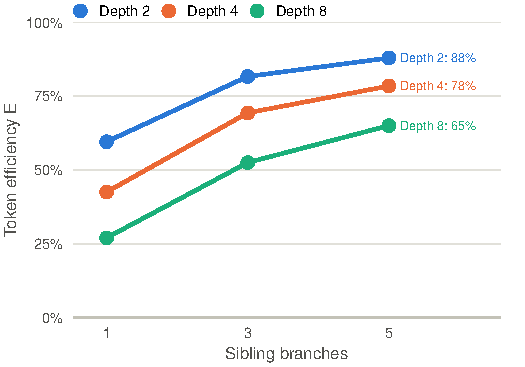
\includegraphics[width=0.75\textwidth]{fig3_efficiency.pdf}
\end{center}

\textbf{What it shows.} Token efficiency $E$ (how much of the full tree ancestor-only leaves out) on the vertical axis, against the number of sibling branches on the horizontal axis. One line per active-path depth. Each point averages 80 scenarios. The whiskers are there but tiny, because $E$ hardly varies within a cell.

\textbf{How to read it.} Higher is a bigger saving. Lines go up to the right: more siblings, more saved. Lines are lower for greater depth: a longer active path means ancestor-only itself is bigger, so the saving is a smaller share.

\begin{example}
Average saving across all scenarios: 62.7\%. Ancestor-only prompts averaged 474 reference tokens against 1,375 for the full tree. Smallest saving: 27.0\% (depth 8, one sibling). Largest: 87.9\% (depth 2, five siblings). The measured saving equalled the siblings' token share in every scenario, as Proposition 1 predicts.
\end{example}

\textbf{In one sentence:} ancestor-only always saves exactly the share of the conversation taken up by side branches, which was 63\% on average and up to 88\%.

\section{Leakage by sibling type (paper Fig.~3)}

\begin{center}
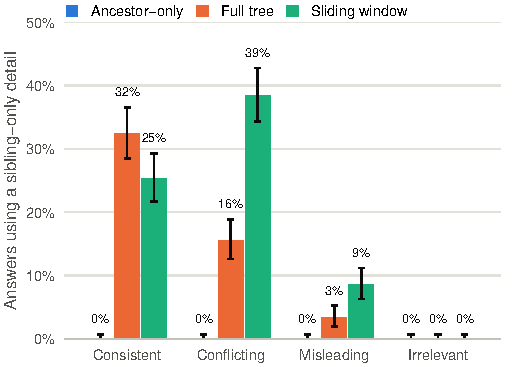
\includegraphics[width=0.75\textwidth]{fig1_leakage.pdf}
\end{center}

\textbf{What it shows.} The share of answers that \emph{used} a detail found only in an abandoned branch (judge-confirmed), for each sibling type and condition. About 540 answers per bar, all three models pooled.

\textbf{How to read it.} Every blue bar is zero: ancestor-only never leaked. Look at orange against green within each group to compare the full tree with the window.

\begin{example}
\begin{center}
\small
\begin{tabular}{@{}lrrr@{}}
\toprule
Sibling type & Ancestor & Full tree & Window \\
\midrule
Consistent & 0\% & 32.4\% & 25.4\% \\
Conflicting & 0\% & 15.6\% & 38.5\% \\
Misleading & 0\% & 3.3\% & 8.5\% \\
Irrelevant & 0\% & 0\% & 0\% \\
\bottomrule
\end{tabular}
\end{center}
\end{example}

\textbf{What the numbers mean.}
\begin{itemize}
\item \textbf{Consistent} siblings leaked most in the full tree. The extra detail is true and fits, so models happily include it (for example, using the column name \texttt{zr\_9fg}).
\item \textbf{Conflicting} siblings leaked much more in the window (38.5\%) than in the full tree (15.6\%). In the full tree, the model can see the real decision and the alternatives side by side and usually picks the real one. In the window, the real decision has often been pushed out, so the alternative is the only answer left. Among window prompts that contained a conflicting value, the model adopted it 86.9\% of the time, against 7.5\% in the full tree.
\item \textbf{Misleading} siblings rarely leaked. Models usually recognised the false claim and rejected it.
\item \textbf{Irrelevant} siblings never leaked. A wiki name or a lunch order number has no reason to appear in an answer about caching.
\end{itemize}

\textbf{The regression's view.} The window leaked $+25.5$ points more than the full tree for conflicting siblings (interval $+20.2$ to $+30.7$), $+2.7$ more for misleading ($+1.2$ to $+4.2$), and $8.2$ points \emph{less} for consistent ($-13.6$ to $-2.8$), all significant after Holm correction. Other factors: leakage rose with depth (OR 7.96 for depth 8 against depth 2) and with late siblings (OR 2.70), and GPT and Mistral leaked much less than Gemini (OR 0.12 and 0.13).

\begin{ask}
\textbf{``Why did deeper conversations leak more?''}\par
A deeper active path means a bigger ancestor-only size, so the window gets a bigger budget and has more room for sibling messages, and the full tree is longer too. The effect is about the baselines; ancestor-only stays at zero at every depth.
\end{ask}

\textbf{In one sentence:} ancestor-only never leaked; the full tree mostly leaked harmless true details, while the window, having lost the real decision, adopted conflicting alternatives in over a third of answers.

\section{Mentioned is not used (paper Fig.~4)}

\begin{center}
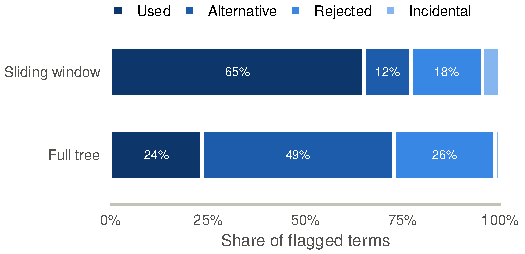
\includegraphics[width=0.75\textwidth]{fig2_term_usage.pdf}
\end{center}

\textbf{What it shows.} Every sibling term the string matcher found in an answer, split by how the leak judge labelled it. Each bar adds up to 100\%. The full-tree bar covers 1,455 terms; the window bar covers 837.

\textbf{How to read it.} The darkest segment (``Used'') is real leakage. The other segments are mentions that do not adopt the term.

\begin{example}
Full tree: used 23.5\%, alternative 49.2\%, rejected 26.0\%, incidental 1.3\%. Window: used 65.0\%, alternative 12.1\%, rejected 18.4\%, incidental 4.5\%.
\end{example}

\textbf{Why it matters.} A study that just searched for sibling terms would have counted more than twice as many full-tree answers as leaking: 29.0\% instead of 12.8\%. The full tree typically \emph{mentions} explored options (``LFU and ARC were only considered'') because it can see the whole history. The window, missing the real decision, \emph{uses} what it sees.

\textbf{In one sentence:} most sibling terms in full-tree answers were mentioned or rejected, not used, so leakage has to be judged, not just searched for.

\section{Correctness by model (paper Fig.~5)}

\begin{center}
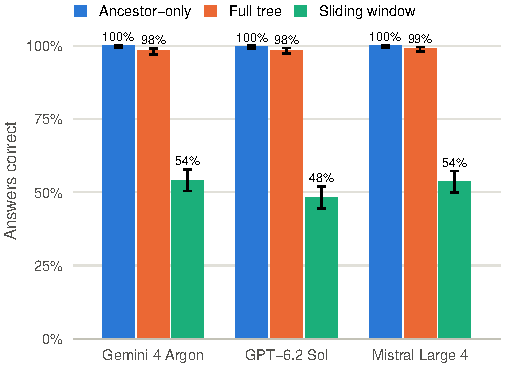
\includegraphics[width=0.75\textwidth]{fig4_correctness.pdf}
\end{center}

\textbf{What it shows.} The share of correct answers (judged measure) for each model and condition. About 720 answers per bar.

\begin{example}
\begin{center}
\small
\begin{tabular}{@{}lrrr@{}}
\toprule
Model & Ancestor & Full tree & Window \\
\midrule
Gemini 4 Argon & 100.0\% & 98.3\% & 54.2\% \\
GPT-6.2 Sol & 99.7\% & 98.5\% & 48.2\% \\
Mistral Large 4 & 100.0\% & 99.0\% & 53.6\% \\
\midrule
All three & 99.9\% & 98.6\% & 52.0\% \\
\bottomrule
\end{tabular}
\end{center}
\end{example}

\textbf{How to read it.} The pattern is the same for every model: ancestor-only and full tree near the top, the window around half. So the finding is about the rules, not one model.

\textbf{In one sentence:} every model answered almost perfectly with ancestor-only or the full tree, and about half the time with an equal-size window.

\section{Quality scores}

\begin{center}
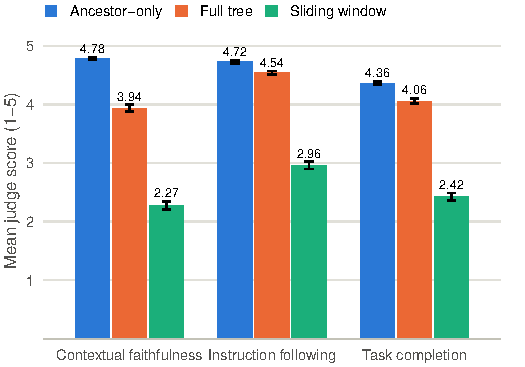
\includegraphics[width=0.75\textwidth]{fig5_quality.pdf}
\end{center}

\textbf{What it shows.} Average judge scores (1 to 5) for each criterion and condition, about 2,160 answers per bar. The paper reports these in Table III.

\begin{example}
\begin{center}
\small
\begin{tabular}{@{}lrrr@{}}
\toprule
Criterion & Ancestor & Full tree & Window \\
\midrule
Contextual faithfulness & 4.78 & 3.94 & 2.27 \\
Instruction following & 4.72 & 4.54 & 2.96 \\
Task completion & 4.36 & 4.06 & 2.42 \\
\bottomrule
\end{tabular}
\end{center}
Paired differences from ancestor-only, with bootstrap intervals: full tree faithfulness $-0.85$ ($-0.92$ to $-0.78$); window faithfulness $-2.51$ ($-2.63$ to $-2.39$). All Holm-adjusted $p < 10^{-6}$.
\end{example}

\textbf{How to read it.} Ancestor-only is highest on every criterion. The full tree loses most on faithfulness: it is usually correct but often brings in details or alternatives that are not part of the conversation being continued. The window loses heavily on everything.

\textbf{In one sentence:} ancestor-only gave the best answers on every quality measure; the full tree was correct but less faithful, and the window was worse on everything.

\section{What the window loses (paper Fig.~6)}

\begin{center}
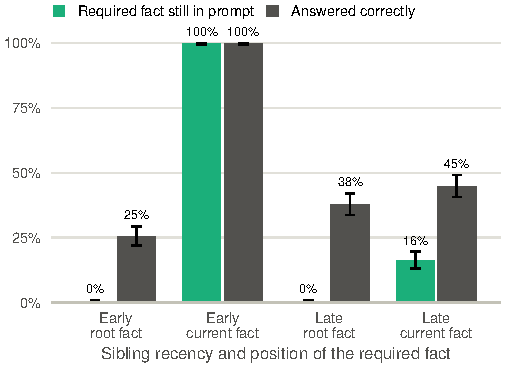
\includegraphics[width=0.75\textwidth]{fig6_window_displacement.pdf}
\end{center}

\textbf{What it shows.} Window answers only, split into the four combinations of sibling recency and fact position. Green bars: the share of prompts that still contained the required fact. Grey bars: the share of answers correct. About 540 answers per group.

\begin{example}
\begin{center}
\small
\begin{tabular}{@{}lrr@{}}
\toprule
Situation & Fact still in prompt & Correct \\
\midrule
Early siblings, fact near root & 0\% & 25.4\% \\
Early siblings, fact near current turn & 100\% & 100.0\% \\
Late siblings, fact near root & 0\% & 37.8\% \\
Late siblings, fact near current turn & 16.1\% & 44.8\% \\
\bottomrule
\end{tabular}
\end{center}
When the fact was still in the window, answers were correct 99.8\% of the time; when it had been pushed out, 32.4\%.
\end{example}

\textbf{How to read it with the formulas.}
\begin{itemize}
\item \textbf{Root, either recency:} 0\% kept. Proposition 5: the root is never in the window when siblings exist.
\item \textbf{Early siblings, current-turn fact:} 100\% kept. The fact is in the newest messages, after the siblings, so the window reaches it first.
\item \textbf{Late siblings, current-turn fact:} 16.1\% kept. The siblings are the newest messages and fill the window first; the fact survives only when the siblings are small (Proposition 6).
\item Answers can still be correct without the fact, mostly when a consistent sibling repeated the right value, or by a lucky guess.
\end{itemize}

\textbf{In one sentence:} the window's errors are almost entirely explained by whether it kept the required fact, exactly as the formulas predict.

\section{The price of ancestor-only (paper Fig.~7)}

\begin{center}
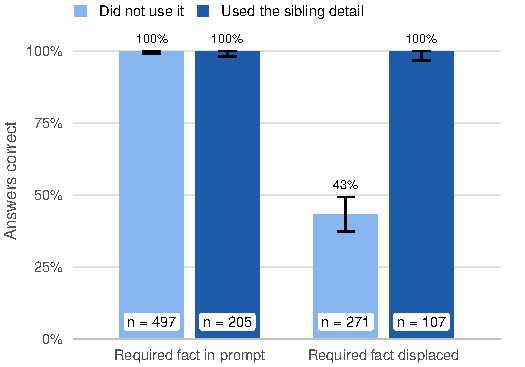
\includegraphics[width=0.75\textwidth]{fig7_consistent_price.pdf}
\end{center}

\textbf{What it shows.} Only answers with a consistent sibling, in the full tree and window. They are split by whether the required fact was still in the prompt (left pair versus right pair) and by whether the answer used the sibling's detail (light versus dark bar). The ``n ='' labels give the number of answers.

\begin{example}
Fact in prompt: 100\% correct whether or not the detail was used. Fact displaced: 43.2\% correct when the detail was not used (271 answers), 100\% when it was (107 answers). Fisher's exact test: $p < 10^{-30}$.
\end{example}

\textbf{What it means.} A consistent sibling restates the correct value (``If we stick with cuid2 keys \dots''). When the window has lost the original decision, that repetition is the only place the model can find the right answer, and using it rescues correctness. This is the one situation where sibling content helps.

\textbf{But:} the judge scored those same answers lower on faithfulness ($-1.28$ points) and task completion ($-0.36$), because they present details that are not in the active path as agreed.

\begin{ask}
\textbf{``So ancestor-only does lose something?''}\par
In principle, yes: a consistent sibling can hold useful information that ancestor-only never sends. In this experiment that only helped when a window had \emph{already} lost the required fact, and under ancestor-only the required fact is always present, so ancestor-only never lost an answer because of it. In real use, a side branch might contain a useful fact that was never stated on the main line; that is the case where combining the active path with retrieval from siblings would help, and it is the paper's suggested future work.
\end{ask}

\section{Robustness: do the results repeat?}

The 73 scenarios run three times show how stable each outcome is. The leakage outcome was identical across all three runs in 91.8\% to 100\% of cases, and correctness in 91.8\% to 100\%, depending on model and condition. Gemini's leakage was fully repeatable, and its correctness changed in a single full-tree scenario. Mistral varied most, consistent with deviation D1.

\textbf{In one sentence:} the results are stable from run to run; the conclusions do not depend on one lucky draw.

\chapter{What it means, and what it does not}

\section{Answering the research question}

\begin{paper}
At an equal token budget, selecting context by tree structure rather than recency removed sibling leakage entirely and kept answer quality on the active path, while the window lost about half of its correct answers.
\end{paper}

Each part of the hypothesis, checked:

\begin{center}
\small
\begin{tabularx}{\textwidth}{@{}XlX@{}}
\toprule
Prediction & Held? & Evidence \\
\midrule
Ancestor-only uses fewer tokens than the full tree & Yes & 62.7\% fewer on average; exactly the siblings' share \\
Both baselines show measurable sibling leakage & Yes & Full tree 12.8\%, window 18.1\% of answers; up to 38.5\% by type \\
Quality preserved when the fact is on the active path & Yes & Ancestor-only 99.9\% correct and highest on all three quality scores \\
\bottomrule
\end{tabularx}
\end{center}

\section{The result that went against expectation}

The literature in your related work says longer, noisier context makes models worse. So you might expect the full tree, the longest prompt, to do worst. It did not. It was nearly as correct as ancestor-only (98.6\% against 99.9\%) and far more correct than the window (52.0\%), which was three times shorter.

\begin{plain}
For this kind of question, \emph{what} is in the prompt mattered far more than \emph{how long} the prompt was. The full tree is long, but it still contains the decision. The window is short, but it may not. A model with the right fact and some clutter does well; a model without the right fact cannot.
\end{plain}

This supports the gap your thesis set out to fill: the earlier study could not separate ``better chosen'' from ``shorter''. Here, the shorter-but-recency-chosen prompt did much worse, so the advantage of branching is about choosing, not just shortening.

\begin{ask}
\textbf{``Doesn't this contradict `context rot' and `lost in the middle'?''}\par
Not really. Those studies show degradation with length, mostly on much longer inputs and on retrieval-style tasks. Your full-tree prompts averaged about 1,400 tokens, short by modern standards, and the full tree still paid a price: lower faithfulness scores and more leakage. At far longer lengths the full tree would likely degrade more. The window's failure is a different mechanism: missing information, not too much information.
\end{ask}

\section{The full tree's real costs}

Correctness alone would make the full tree look nearly as good as ancestor-only. It is not, for three reasons:
\begin{enumerate}
\item \textbf{Three times the tokens}, and the gap grows over a long session (Proposition 2).
\item \textbf{Leakage}: 12.8\% of full-tree answers used an abandoned-branch detail, rising to 32.4\% with consistent siblings.
\item \textbf{Lower quality}: faithfulness 3.94 against 4.78, because the answers bring in explored options and details that are not part of the conversation being continued.
\end{enumerate}

\section{The price of ancestor-only}

\begin{paper}
Ancestor-only prompting has a measurable price only when a consistent sibling carries information the active path has lost, and in this benchmark that happened only after the window displaced it.
\end{paper}

Your thesis framed this as a falsifiable test: if consistent-sibling leakage improved quality in the baselines, ancestor-only would have a measurable price. The answer is nuanced. Using a consistent detail rescued correctness when the window had lost the fact, which is a real benefit. But it lowered the judge's quality scores, and under ancestor-only the fact is never lost. So in this benchmark ancestor-only paid no price in correctness. A real conversation could hold useful information only in a side branch; that is the case for future work on retrieving from siblings.

\section{Limitations, in your words}

Be ready to state these yourself before anyone asks.

\begin{enumerate}
\item \textbf{Synthetic, template-based conversations with forced-choice answers.} Clean measurement, but real conversations are messier and answers are often not a single word. Absolute rates may not transfer; the direction of the comparison is more likely to.
\item \textbf{Three models.} From three different families, and the pattern held for all three, but other models could behave differently.
\item \textbf{Temperature.} GPT-6.2 Sol could not be set to temperature 0, and Mistral was not fully repeatable. Both were measured by the repeat runs.
\item \textbf{An LLM judge.} Quality and the used/mentioned labels come from one model. It is blind to the condition and from a different family, and the human review measures its agreement with a person. Its rubric penalizes true details absent from the active path, which matters for consistent siblings.
\item \textbf{Exposure in the window.} Planted facts were placed early in each sibling branch, so they were often outside the window. Window leakage is therefore measured among exposed calls, a smaller set than for the full tree.
\item \textbf{One question per scenario.} The experiment tests the moment of asking, not a whole session; the cost growth over a session is shown mathematically (Proposition 2), not measured.
\end{enumerate}

\section{What you can and cannot claim}

\textbf{You can say:}
\begin{itemize}
\item At an equal token budget, choosing context by tree structure beat choosing by recency on leakage, correctness and judged quality, for three models from different families.
\item Ancestor-only produced no sibling leakage (0 of 2,160; at most 0.17\%).
\item The window's failures follow mathematically from how a recency window works on a branched conversation, and every prediction held.
\item String matching alone overstates leakage; judging how terms are used is necessary.
\end{itemize}

\textbf{You should not say:}
\begin{itemize}
\item That ancestor-only is always best. When useful information lives only in a side branch, it cannot use it.
\item That the full tree is ``wrong''. It was nearly as correct; its costs were tokens, leakage and quality.
\item That the exact percentages apply to real users' chats. They come from synthetic conversations.
\end{itemize}

\chapter{Defending it: questions and answers}

These are the questions an examiner or advisor is most likely to ask, with answers you can give in your own words. Practise saying them aloud; do not memorise them word for word.

\section*{About the idea}

\textbf{Q1. What problem does your thesis solve?}\par
When people explore alternatives in a chat with an AI, the abandoned explorations stay in the prompt. That wastes tokens and can mislead the model. I tested whether sending only the conversation's active path, as Traceback does, fixes this better than the common alternative of sending the most recent messages, at the same prompt size.

\textbf{Q2. Isn't it obvious that sending less irrelevant text is better?}\par
That part was already shown by earlier work. What was not known is whether the benefit comes from \emph{choosing} the right messages or simply from sending fewer. My equal-budget window separates those: it sends exactly as many tokens as ancestor-only but chooses by recency, and it did much worse.

\textbf{Q3. What is new compared with the earlier branching study?}\par
Three things: an equal-budget comparison, sibling type as a controlled variable (including consistent and misleading siblings, which they did not test), and a short formal analysis whose predictions I checked scenario by scenario.

\section*{About the method}

\textbf{Q4. Why synthetic conversations?}\par
So that every fact is planted on purpose and the correct answer and every possible leak are known exactly. With real chats I could not tell which facts only lived in abandoned branches. The cost is realism, which I list as a limitation.

\textbf{Q5. How do you know a leak really came from the sibling?}\par
Every sibling-only detail carries a random canary, such as \texttt{orbit\_y5y}, that no model could guess. On ancestor-only prompts, which never contain sibling content, the detector found 0 canaries in 2,598 answers, so false alarms are essentially zero. For forced-choice values like ``LRU'', which a model could guess, I only count a leak when the value was actually in the prompt.

\textbf{Q6. Why did you need a judge for leakage at all?}\par
Because finding a term is not the same as using it. Many full-tree answers said things like ``we chose LRU; LFU was only explored''. The judge labelled each term as used, mentioned as an alternative, rejected or incidental. Only 23.5\% of the terms found in full-tree answers were actually used.

\textbf{Q7. Why trust an AI judge?}\par
It is from a different model family than any model tested, it never sees the condition or model, and answers are judged in shuffled order. I also scored 150 answers myself, blind, and report Cohen's kappa between my scores and the judge's. I acknowledge its rubric penalizes true details not on the active path.

\textbf{Q8. Why only three models?}\par
Budget and scope. I chose one frontier, one mid-size and one open-weights model from three different companies so the result is not about one family. The pattern was the same for all three.

\textbf{Q9. GPT could not be run at temperature 0. Is that a problem?}\par
It reduces repeatability, which I measured directly with three runs of 73 scenarios. GPT's leakage outcome was identical across runs in at least 98.6\% of cases. The conclusions hold for the two models that were run at temperature 0 as well.

\textbf{Q10. Why did you change the correctness measure?}\par
I did not change the definition. My brief defines correct as ``the required value is present and no conflicting value is asserted''. The first implementation counted any mention of a conflicting value as asserting it. Reading answers showed this was wrong, so I used the leak judge's labels to separate assertions from mentions. I report both. The change helped the full tree, a baseline, not my method, and ancestor-only is most correct under both.

\textbf{Q11. Some Mistral answers were re-run. Isn't that cherry-picking?}\par
No. 107 Mistral answers were cut off because the model used up its output allowance on reasoning, slightly more often under ancestor-only. I re-sent exactly those prompts, byte for byte, with a bigger allowance, and recorded it as a documented deviation. Leaving them as failures would have biased the results \emph{against} ancestor-only.

\textbf{Q12. How do I know you didn't adjust the dataset after seeing results?}\par
The dataset was hashed and tagged in git before the full run, and it regenerates from its seed with the identical hash. Every model response and judgment is saved in the repository.

\section*{About the results}

\textbf{Q13. What was your most important result?}\par
At the same size, the recency window was correct only 52.0\% of the time, while ancestor-only was correct 99.9\% of the time and never leaked. The window fails because it always drops the oldest messages first, which is exactly where early decisions live.

\textbf{Q14. The full tree was 98.6\% correct. So why not just send everything?}\par
Because it costs three times the tokens, and that grows over a session; 12.8\% of its answers used abandoned-branch details; and its answers were judged less faithful (3.94 against 4.78). Ancestor-only matched its correctness without any of those costs.

\textbf{Q15. Why did the window leak conflicting values so much more than the full tree?}\par
When the full tree sees ``we chose LRU'' and ``what about LFU?'', it usually picks the real decision. The window often no longer contains ``we chose LRU'', so LFU is the only option in front of it. Given exposure, it adopted the conflicting value 86.9\% of the time, against 7.5\% for the full tree.

\textbf{Q16. Why did deeper conversations leak more?}\par
A deeper active path makes the ancestor-only prompt bigger, which gives the window a bigger budget with more room for sibling messages, and makes the full tree longer. Ancestor-only stays at zero regardless.

\textbf{Q17. Is there any case where ancestor-only is worse?}\par
In principle yes: if a side branch contains useful information that was never stated on the main line, ancestor-only cannot use it. My consistent-sibling analysis shows such information can rescue an answer, but in my benchmark that only happened after the window had lost the fact, which never happens under ancestor-only. That case motivates future work on retrieving from siblings.

\section*{About the theory}

\textbf{Q18. Explain Proposition 1 in one sentence.}\par
The share of tokens ancestor-only saves is exactly the share of the conversation taken up by side branches, because the conversation is just the active path plus the side branches.

\textbf{Q19. Why is the first message never in the window?}\par
The window keeps a message only if it and everything newer fit in the budget. For the first message, ``everything newer'' is the whole conversation, which is bigger than the active path whenever side branches exist, and the budget equals the active path.

\textbf{Q20. What does ``exposure times uptake'' mean?}\par
A model can only use a sibling fact beyond chance if the fact is in its prompt. Whether it is in the prompt (exposure) is decided by the tree and the rule, without any model. What the model does with it (uptake) is what the experiment measures.

\textbf{Q21. Did you test the theory?}\par
Yes. The token saving matched the formula in all 720 scenarios. The test for which messages the window keeps was right in 720 of 720. The root fact was never in the window (0 of 360). The late-sibling survival condition was right in 360 of 360.

\section*{About Traceback and practice}

\textbf{Q22. Does the experiment really test Traceback's code?}\par
Yes. The scenarios were loaded into Traceback's own database schema, and a test reads the exact recursive SQL from Traceback's source and confirms the experiment's ancestor-only prompts are identical to what Traceback produces, and to its own lineage function.

\textbf{Q23. What should builders of branching chat tools take from this?}\par
Choose context by the conversation tree, not by recency. Recency windows drop early decisions and then adopt whatever alternatives are left. If you need information from side branches, retrieve it deliberately rather than including it by recency.

\textbf{Q24. What would you do next?}\par
Test real conversations rather than templates; add free-form answers; measure cost over whole sessions; and test combining the active path with selective retrieval from sibling branches.

\textbf{Q25. What would change your conclusion?}\par
If, on real conversations, useful information lived in side branches often enough that ancestor-only lost more answers than it saved. The consistent-sibling analysis is the start of testing that.

\chapter{Decision log}

Every significant decision, in the order it was made, with the reason. Use this when someone asks ``why did you do it that way?''

{\small
\begin{xltabular}{\textwidth}{@{}p{3.6cm}XX@{}}
\toprule
Decision & Why & Alternative considered \\
\midrule
\endhead
Separate experiment database (new Neon project) & Never touch production data; a branch of production would copy real users' chats & Branch of production DB; local Postgres \\
Safety guard with a production deny list & Every script refuses to run unless the database is the experiment one & None; required by your brief \\
Reuse Traceback's schema, client and SQL & Evaluate the production rule, not an imitation & Rewrite the queries in the experiment \\
Six domains, seven options each & Results not tied to one topic; enough wrong options for five conflicting siblings & Fewer domains \\
Forced-choice answers & Correctness checkable automatically & Free-form answers judged by a model \\
Siblings fork at exchange $\lfloor d/2 \rfloor$ & Makes root versus current-turn fact position meaningful & Fork from root, or from last message \\
Question asked at $\max(t)+1$ & User returns to the main line after exploring; full tree includes late siblings & Ask at the ask node's time \\
Template filler, no LLM rewrite & Planted facts stay exactly in place; fully reproducible & LLM paraphrase of filler \\
Canary in each sibling's first exchange (kept) & Your choice after the dry run; analyse window leakage conditional on exposure & Move canaries to the last exchange \\
Window budget = ancestor-only size & Isolates choosing from size & Fixed budget for all \\
Whole messages only in the window & Never cut a message mid-sentence & Truncate the last message \\
Gemini, GPT, Mistral under test; Claude Opus as judge & Three families; judge from a fourth & Other model sets \\
Each model pinned to one provider, no fallbacks & Same hardware and precision for every call & Default routing \\
Lowest reasoning, 1,024-token cap & Same setting for all; low cost & Default reasoning \\
10\% of scenarios run 3 times & Measure run-to-run variance & No repeats \\
D1: replay 107 cut-off Mistral calls at 4,096 & Avoid bias against ancestor-only; same prompts byte for byte & Count as failures \\
Leak judge on flagged answers & String matching counts mentions and rejections as leaks & String matching only \\
Quality judge sees only active path, question, answer & Blind to condition & Show full context \\
Transcript with plain speaker labels & OpenRouter's guardrail blocked bracketed role tags & None \\
Judged correctness as main measure & Matches the brief's ``asserted'' definition & Strict string rule only (reported as a check) \\
Model as a fixed effect & Only three models & Random effect (as in brief) \\
Exact intervals for zero-leak cells & Logistic regression cannot estimate zero cells & Force them into the model \\
Scenario-cluster bootstrap & Keeps each scenario's answers together & Resample individual answers \\
Holm correction within families & Control false positives from many tests & No correction; Bonferroni \\
Human sample of 150, stratified & Validate the judge; enough for a useful kappa & Smaller sample; second AI judge \\
\bottomrule
\end{xltabular}
}

\appendix
\chapter{Glossary}

\begin{description}[style=nextline,leftmargin=0pt,font=\bfseries]
\item[Active path] The messages from the root down to the current message: the ask node and all its ancestors. Written $A(a)$.
\item[Ancestor] A message's parent, its parent's parent, and so on to the root.
\item[Ancestor-only prompting] Sending only the active path to the model. Traceback's rule; condition ``ancestor''.
\item[API] A way for one program to call another over the internet.
\item[Ask node] The last message before the final question. Written $a$.
\item[Bootstrap] Getting a confidence interval by resampling the data many times.
\item[Budget ($B$)] The window's token limit, equal to the active path's weight.
\item[Canary] A random, unguessable string planted in a sibling branch to detect leaks.
\item[Cell] One combination of the five controlled variables; 144 in total.
\item[Chance hit] A sibling value in an answer that was not in the prompt; a guess, not a leak.
\item[Clopper--Pearson interval] An exact confidence interval for a rate.
\item[Cohen's kappa] Agreement between two raters, corrected for chance.
\item[Complete separation] When a group has no positive outcomes, so logistic regression cannot estimate it.
\item[Condition] One of the three context rules: ancestor-only, full tree, sliding window.
\item[Confidence interval] A range that very plausibly contains the true value; 95\% here.
\item[Consistent sibling] A side branch that agrees with the main decision and adds a true detail.
\item[Conflicting sibling] A side branch that chooses a different option.
\item[Context window] The maximum number of tokens a model can read at once.
\item[Correct (judged)] States the required value and does not assert a conflicting one (judge decides).
\item[Correct (strict)] States the required value and contains no conflicting value at all.
\item[CTE, recursive] A SQL query that repeats a step; used to climb from a message to the root.
\item[Depth] Number of steps from the root; also the number of active exchanges before the question.
\item[Deviation D1] The documented re-run of 107 cut-off Mistral calls.
\item[Difference-in-differences] How much one factor's effect changes across levels of another.
\item[Exchange] One user message and the assistant's reply.
\item[Exposure ($X_c$)] Whether a sibling fact is in a rule's prompt.
\item[Fisher's exact test] Exact test of association in a 2-by-2 table.
\item[Fork point] The active message the sibling branches split from; exchange $\lfloor d/2 \rfloor$.
\item[Full tree] Sending every message, in time order. Condition ``full\_tree''.
\item[Hash (sha256)] A fingerprint of a file; proves it did not change.
\item[Holm correction] An adjustment of p-values for running many tests.
\item[Irrelevant sibling] A side branch about an unrelated topic.
\item[Judge] Claude Opus 5.5, used to label leaks and score quality.
\item[Leakage] The answer uses (not just mentions) a detail found only in a sibling branch.
\item[Logical clock ($\tau$)] Whole numbers giving the order messages were written.
\item[Logistic regression] Regression for yes/no outcomes; effects reported as odds ratios.
\item[Misleading sibling] A side branch with a plausible but false claim.
\item[Mixed model] A regression with fixed effects and random effects (here, per scenario).
\item[Odds, odds ratio] $p/(1-p)$; and the ratio of two odds.
\item[OpenRouter] A service that gives one API for many models.
\item[p-value] How surprising a result would be if there were no real difference.
\item[Provider] The company that actually runs a model for OpenRouter.
\item[Reference tokenizer] \texttt{o200k\_base}, used to count tokens the same way for all models.
\item[Risk difference] The difference between two rates, in percentage points.
\item[Root] The first message ($r$).
\item[Scenario] One synthetic test conversation with a known answer.
\item[Sibling, sibling branch] A branch not on the active path; $S(a)$ is all sibling content.
\item[Sliding window] Sending the newest whole messages up to the budget. Condition ``window''.
\item[Suffix sum] A message's weight plus the weight of every newer message.
\item[System prompt] The fixed instruction at the start of every prompt.
\item[Temperature] A randomness setting; 0 is as repeatable as possible.
\item[Token] A chunk of text that models read; about three quarters of a word.
\item[Token efficiency ($E$)] The share of the full tree's tokens that ancestor-only leaves out.
\item[Uptake ($u_c$)] How often a model uses a sibling fact when it is in the prompt.
\item[Weight ($w$)] A message's token count under the reference tokenizer.
\item[Wilcoxon signed-rank test] A paired test that does not assume a bell curve.
\end{description}

\chapter{Reproducing everything}

Everything lives on the \texttt{thesis/experiment} branch in \texttt{thesis-experiments/}. Each phase has commands that regenerate its output from the frozen data.

\section{Where things are}

\begin{center}
\small
\begin{tabularx}{\textwidth}{@{}lX@{}}
\toprule
Path & What it holds \\
\midrule
\texttt{config/experiment.yaml} & Design levels, seed, models, cost cap, analysis decisions \\
\texttt{generator/} & Scenario templates, generator and validator \\
\texttt{data/scenarios.jsonl} & The 720 frozen scenarios (sha256 in \texttt{scenarios.sha256}) \\
\texttt{loader/} & Safety guard, migrations, loading into Traceback's database \\
\texttt{builders/context.ts} & The three context rules \\
\texttt{runner/} & Model calls, cost cap, resume, replay for D1 \\
\texttt{results/raw/} & Every model call: prompt, answer, tokens, cost, exposure \\
\texttt{scoring/} & Leak detection, judge prompts and runner, human sample \\
\texttt{results/scored/} & Deterministic scores and all judge outputs \\
\texttt{analysis/} & Results table, statistics (R) and figures (R) \\
\texttt{results/analysis/} & \texttt{answers.csv}, \texttt{stats.txt}, \texttt{stats.json} \\
\texttt{results/figures/} & Figures (titled and IEEE-column versions) \\
\texttt{docs/paper/} & The IEEE paper \\
\texttt{docs/companion/} & This book \\
\texttt{DEVIATIONS.md} & Every change to the plan after the freeze \\
\bottomrule
\end{tabularx}
\end{center}

\section{Commands}

\begin{lstlisting}
# verify the frozen dataset
shasum -a 256 -c data/scenarios.sha256
# rebuild the results table, statistics and figures
python3 -I analysis/build_table.py
Rscript analysis/models.R
Rscript analysis/figures.R
# rebuild the paper and this book
cd docs/paper && tectonic -X compile paper.tex
cd ../companion && tectonic -X compile companion.tex
\end{lstlisting}

Model calls and judgments are not re-run by these commands: they cost money and are saved in \texttt{results/raw} and \texttt{results/scored}. Re-running them would produce close but not identical answers, which is why the saved files are the record.


\end{document}
